\subsection{离散赋值}

定义 3. 设 K 是一个（未必交换的）域，v 是 K 上的一个赋值，\(\Gamma\) 是 v 的阶群。若存在由有序群 \(\Gamma\) 到 Z 上的一个（必然唯一的）同构，则称 v 为离散的。设 \(\gamma\) 是在此同构下对应于 1 的 \(\Gamma\) 的元素；K 中满足 \(v(u) = \gamma\) 的每个元素 u 都称为 v 的一个单值化元。若离散赋值的阶群为 Z，则称它是赋范的。

例如，由主理想整环*或因子分解整环*的极端元 p 所定义的赋值 \(v_{p}\) 是一个赋范离散赋值，它以 p 为单值化元。特别地，若 k 是域，则 \(k[[T]]\) 是 \(k((T))\) 上一个离散赋值的环，该赋值以 T 为单值化元。* 设 S 是一维连通复解析空间，K 是 S 上的亚纯函数域，\(z_{0}\) 是 S 的一点；\(f \in K\) 中在 \(z_{0}\) 处全纯的函数组成的集合是某个离散赋值 v 的环；函数 \(f \in K\) 是 v 的单值化元，当且仅当它在 \(z_{0}\) 处全纯且取值为零，并且存在 \(z_{0}\) 在 S 中的一个邻域 V，使 f 在 V 上的限制是 V 到 C 中原点的某邻域上的一个同胚。正是这个例子以及其他类似的例子成为“单值化元”一词的来源。*

命题 8. 设 K 是一个（未必交换的）域，v 是 K 上的一个离散赋值，A 是 v 的环，u 是 v 的一个单值化元。A 的非零理想都是双侧理想，且形如 Au \(^{n}\)（n ≥ 0）。

可以假定 \(v\) 是赋范的，于是 \(v(u) = 1\) 。对一切 \(x \in \mathbf{K}^*\) ，存在整数 \(n \in \mathbf{Z}\) 使得 \((v(x) = n = v(u^n))\)，从而可以写出

\[
x = z u ^ {n} = u ^ {n} z ^ {\prime},
\]

其中 \(z, z'\) 是环 A 的两个可逆元；由此即得命题。

命题 9. 设 A 是一个与其分式域不同的局部整环。下列条件等价：

\begin{enumerate}
\def\labelenumi{(\alph{enumi})}
\item
  A 是一个离散赋值的环。
\item
  A 是主理想整环。
\item
  理想 \(\mathfrak{m}(\mathbf{A})\) 是主理想，且 \(\bigcap_{n=1}^{\infty} \mathfrak{m}(\mathbf{A})^n = (0)\) 。
\item
  A 是 Noether 环，且 \(\mathfrak{m}(\mathbf{A})\) 是主理想。
\item
  A 是 Noether 赋值环。
\end{enumerate}

命题 8 表明 (a) 蕴含 (b)、(d) 与 (e)。若 A 是主理想整环，则由于 A 是局部环（《代数》第七章 §1 第 3 节定理 2），\(\mathfrak{m}(\mathbf{A}) = \mathbf{A}\mathbf{u}\)，且 A 的每个非零理想都形如 \(\mathbf{A}\mathbf{u}^n\)；因此 \(\bigcap_{n=1}^{\infty} \mathfrak{m}(A)^n = 0\) ；这表明 (b) 蕴含 (c)。另一方面，(d) 蕴含 (c)（第三章 §3 第 2 节命题 5 的推论）；由 §1 第 4 节命题 2，(c) 蕴含 (a)。于是条件 (a)、(b)、(c)、(d) 等价并且蕴含 (e)。最后假设 (e) 成立，我们来证明 (b) 成立；只需证明下面的引理：

引理 1. 设 A 是赋值环。每个有限生成的无扭 A-模都是自由模。A 的每个有限生成理想都是主理想。每个无扭 A-模都是平坦模。

设 E 是有限生成的无扭 A-模，\(x_{1}, \ldots, x_{n}\) 是 E 的一组个数最少的生成元；我们证明它们线性无关。若 \(\sum_{i=1}^{n} a_i x_i = 0\)（ \(a_i \in A\) ）是 \(x_i\) 之间的一个非平凡关系，则某个 \(a_i\)（例如 \(a_1\)）整除其余所有的元素，因为 \(A\) 的主理想集合按包含关系是全序的（§ 1 第 2 节定理 1）；又因该关系非平凡，故 \(a_1 \neq 0\)。由于 \(E\) 无扭，可以用 \(a_1\) 去除，这相当于假定 \(a_1 = 1\) 。但这样 \(x_1\) 就是 \(x_2, \ldots, x_n\) 的线性组合，与 \(n\) 的最小性相矛盾。因此 \(E\) 是自由的。

特别地，A 的每个有限生成理想 a 都是主理想，因为 a 的某个生成系中的所有元素都是其中一个的倍数。于是《代数》第一章 § 2 第 4 节命题 3 表明每个无扭 A-模都是平坦模。

\section{赋值的高}

\subsection{同一域的赋值环的包含}

命题 1. 设 K 是域，A 是 K 的一个赋值环。那么：

\begin{enumerate}
\def\labelenumi{(\alph{enumi})}
\item
  每个环 \(\mathbf{B}\) ，只要它满足 \(\mathbf{A} \subset \mathbf{B} \subset \mathbf{K}\) ，就是 \(\mathbf{K}\) 的赋值环；
\item
  这种环的极大理想 \(\mathfrak{m}(\mathbf{B})\) 含于 \(\mathbf{A}\)，且它是 \(\mathbf{A}\) 的素理想；
\item
映射 \(\mathfrak{p} \mapsto \mathbf{A}_{\mathfrak{p}}\) 是由 \(\mathbf{A}\) 的素理想集合到环 \(\mathbf{B}\) （满足 \(\mathbf{A} \subset \mathbf{B} \subset \mathbf{K}\) ）的集合上的一个递减双射；其逆双射是映射 \(\mathbf{B} \mapsto \mathfrak{m}(\mathbf{B})\) 。
\end{enumerate}

设 B 是满足 \(A \subset B \subset K\) 的环且 \(x \in K - B\) ，则 \(x \in K - A\) ，于是 \(x^{-1} \in \mathfrak{m}(A) \subset B\) ，这同时证明了 B 是 K 的赋值环以及 \(\mathfrak{m}(B) \subset \mathfrak{m}(A)\) ；由于 \(\mathfrak{m}(B) = \mathfrak{m}(B) \cap A\) 是 A 的素理想，我们已证明了 (a)

与 (b)。此外，\(\mathbf{A}_{\mathfrak{m}(\mathbf{B})} \subset \mathbf{B}\) ；反之，若 \(x \in \mathbf{B} - \mathbf{A}\) ，则 \(x^{-1} \in \mathbf{A}\) 且 \(x^{-1} \notin \mathfrak{m}(\mathbf{B})\) ，因此 \(x \in \mathbf{A}_{\mathfrak{m}(\mathbf{B})}\) ；于是 \(\mathbf{A}_{\mathfrak{m}(\mathbf{B})} = \mathbf{B}\) 。最后设 \(\mathfrak{p}\) 是 \(\mathbf{A}\) 的素理想；记 \(\mathbf{B} = \mathbf{A}_{\mathfrak{p}}\) ；则 \(\mathfrak{m}(\mathbf{B}) \cap \mathbf{A} = \mathfrak{p}\) （第二章 §2 第 5 节命题 11），且由 (b) 有 \(\mathfrak{m}(\mathbf{B}) \subset \mathbf{A}\) ；因此 \(\mathfrak{m}(\mathbf{B}) = \mathfrak{p}\) ，这表明命题中的映射 \(\mathfrak{p} \mapsto \mathbf{A}_{\mathfrak{p}}\) 与 \(\mathbf{B} \mapsto \mathfrak{m}(\mathbf{B})\) 是互逆的双射。

推论. K 中含 A 的子环的集合按包含关系是全序的。

A 的素理想集合按包含关系是全序的（§ 1 第 2 节定理 1 (e)），且映射 \(\mathfrak{p} \mapsto \mathrm{A}_{\mathfrak{p}}\) 反转包含关系。

命题 2. 设 K 是域，B 是 K 的一个赋值环，\(h_B\) 是与 B 相伴的 K 的位（取值于 \(\kappa(B)\) ）。那么映射 \(A \mapsto h_B(A)\) 定义了由含于 B 的 K 的赋值环组成的集 \(\mathfrak{A}\) 到 \(\mathfrak{A}'\) （\(\kappa(B)\) 的赋值环组成的集）上的一个双射。

若 \(\mathbf{A} \in \mathfrak{A}\) ，则 \(h_{\mathrm{B}}(\mathbf{A}) \in \mathfrak{A}'\) ：因为若 \(x' = h_{\mathrm{B}}(x)\) （其中 \(x \in \mathbf{B}\) ）是 \(\kappa(\mathbf{B}) - h_{\mathrm{B}}(\mathbf{A})\) 的元素，则 \(x \notin \mathbf{A}\) ，于是 \(x^{-1} \in \mathbf{A}\) ，且 \(h_{\mathrm{B}}(x)^{-1} \in h_{\mathrm{B}}(\mathbf{A})\) 。另一方面，对 \(\mathbf{A} \in \mathfrak{A}\) 有 \(\mathbf{A} \supset \mathfrak{m}(\mathbf{B})\) （命题 1 (b)），因此映射 \(\mathbf{A} \mapsto h_{\mathrm{B}}(\mathbf{A})\) 是单射。最后，设 \(\mathbf{A}' \in \mathfrak{A}'\) ，\(\mathbf{A} = \bar{h}_{\mathrm{B}}^{-1}(\mathbf{A}') \subset \mathbf{B}\) ；我们将证明 \(\mathbf{A} \in \mathfrak{A}\) ，从而完成证明；若 \(x \in \mathbf{K} - \mathbf{A}\) ，则或者 \(x \notin \mathbf{B}\) ，或者 \(x \in \mathbf{B}\) ；若 \(x \notin \mathbf{B}\) ，则 \(x^{-1} \in \mathfrak{m}(\mathbf{B}) \subset \mathbf{A}\) ；若 \(x \in \mathbf{B}\) ，则 \(h_{\mathrm{B}}(x) \in \kappa(\mathbf{B})\) 且 \(h_{\mathrm{B}}(x) \notin \mathbf{A}'\) ，于是 \(h_{\mathrm{B}}(x^{-1}) \in \mathbf{A}'\) ，我们再次得出 \(x^{-1} \in \mathbf{A}\) ；因此 \(\mathbf{A} \in \mathfrak{A}\) 。

推论. 设 A 与 B 是 K 的两个赋值环，其中 \(A \subset B\) ；设 \(A' = h_{B}(A)\) ，它是 \(\kappa(B)\) 的一个赋值环。\(\kappa(A')\) 是 \(A'\) 的剩余域，它典范地同构于 A 的剩余域 \(\kappa(A)\) ，且与 A 相伴的位 \(h_{A}\) 是 \(h_{A'} \circ h_{B}\) （与 \(A'\) 和 B 相伴的位的复合）。

由于局部环 A' 是局部环 A 的一个商，它们的剩余域典范地同构，且等式 \(h_{\mathrm{A}}(x) = h_{\mathrm{A}'}(h_{\mathrm{B}}(x))\) 对 \(x \in A\) 成立。另一方面，若 \(x \in B - A\) ，则 \(h_{\mathrm{B}}(x) \notin A'\) ，等式两边都等于 \(\infty\) ；若 \(x \in K - B\) ，情形相同。

注. 反之，设 \(f\) 是 \(\mathbf{K}\) 的一个取值于 \(\mathbf{K}'\) 的位，\(f'\) 是 \(\mathbf{K}'\) 的一个取值于 \(\mathbf{K}''\) 的位。那么 \(f' \circ f\) 是 \(\mathbf{K}\) 的一个位，它的环含于位 \(f\) 的环。

\subsection{有序群的孤立子群}

为了从赋值的观点研究第 1 节中的情形，我们需要下面的定义 1 和命题 3。

定义 1. 有序群 G 的子群 H 称为孤立的，如果关系 \(0 \leqslant y \leqslant x\) 与 \(x \in \mathbf{H}\) 蕴含 \(y \in \mathbf{H}\) 。

例 (1) 设 A 与 B 是两个有序群；给 \(A \times B\) 赋以字典序（即~“ \((a, b) \leqslant (a', b')\) ”等价于“ \((a < a')\) 或 \((a = a' \text{ 且 } b \leqslant b')\) ”）。立即可见，\(A \times B\) 的第二个因子 B 是 \(A \times B\) 的孤立子群。

命题 3. 设 G 是有序群，P 是其正元素集合。

\begin{enumerate}
\def\labelenumi{(\alph{enumi})}
\item
  由 G 到某个有序群的递增同态的核是 G 的孤立子群。
\item
  反之，设 H 是 G 的孤立子群，g 是 G 到 G/H 上的典范同态。那么 \(g(P)\) 是 G/H 上某个有序群结构的正元素集合。此外，若 G 是全序的，则 G/H 也是全序的。
\item
  设 \(f\) 是由 \(G\) 到某个有序群的递增同态；设 \(H\) 表示 \(f\) 的核。若 \(0 \leqslant y \leqslant x\) 且 \(x \in H\) ，则 \(0 \leqslant f(y) \leqslant f(x) = 0\) ，于是 \(f(y) = 0\) ，即 \(y \in H\) 。因此 \(H\) 是孤立的。
\item
  设 \(\mathbf{H}\) 是 \(\mathbf{G}\) 的孤立子群，\(g\colon \mathbf{G}\to \mathbf{G} / \mathbf{H}\) 。设 \(\mathbf{P}' = g(\mathbf{P})\) 。显然 \(\mathbf{P}' + \mathbf{P}'\subset \mathbf{P}'\) 。并且
\end{enumerate}

\[
\mathrm{P} ^ {\prime} \cap (- \mathrm{P} ^ {\prime}) = \{0 \},
\]

因为，若 \(x\) 与 \(y\) 是 \(\mathbf{P}\) 中满足 \(g(x) = -g(y)\) 的元素，则 \(x + y \in \mathbf{H}\) ，于是 \(x \in \mathbf{H}\) 且 \(y \in \mathbf{H}\) ，因为 \(\mathbf{H}\) 是孤立的；因此 \(g(x) = g(y) = 0\) 。这样，\(\mathbf{P}'\) 是 \(\mathbf{G} / \mathbf{H}\) 上某个有序群结构的正元素集合（《代数》第六章 §1 第 3 节命题 3）。最后，若 \(\mathbf{G}\) 是全序的，则 \(\mathbf{P} \cap (-\mathbf{P}) = \mathbf{G}\) ，于是 \(\mathbf{P}' \cup (-\mathbf{P}') = \mathbf{G} / \mathbf{H}\) ，因此 \(\mathbf{G} / \mathbf{H}\) 是全序的（同前）。

例 (2) 若重新考察 G 是字典积 \(A \times B\) 且 H = B 的例子，则有序群 G/H 典范地等同于 A。

\subsection{赋值的比较}

设 K 是域，A 是 K 的一个赋值环。对 K 中含 A 的每个子环 B，有 \(U(A) \subset U(B)\) 。于是存在一个典范同态 \(\lambda\) ，它由 \(\Gamma_{A} = K^{*}/U(A)\) 映到 \(\Gamma_{B} = K^{*}/U(B)\) 上，其核为 \(U(B)/U(A)\) 。设 \(v_{A}\) 与 \(v_{B}\) 分别表示由 A 与 B 定义的 K 上的典范赋值（ \(\S 3\) 第 2 节），则

\[
v _ {\mathrm{B}} = \lambda \circ v _ {\mathrm{A}}.\tag{1}
\]

由于 \(A \subset B\) ，\(\lambda\) 把 \(\Gamma_{A}\) 的正元素映到 \(\Gamma_{B}\) 的正元素，因此是递增的。于是（命题 3）\(H_{B}\) 作为 \(\lambda\) 的核，是 \(\Gamma_{A}\) 的孤立子群，并且 \(\lambda\) 分解为 \(\Gamma_{A} \to \Gamma_{A}/H_{B} \xrightarrow{\mu} \Gamma_{B}\) ，其中 \(\mu\) 是递增的双射同态，因而是全序群的同构；因此 \(\Gamma_{B}\) 等同于商全序群 \(\Gamma_{A}/H_{B}\) 。

命题 4. 映射 \(\mathbf{B} \mapsto \mathbf{H}_{\mathbf{B}}\) 是由 \(\mathbf{K}\) 中含 \(\mathbf{A}\) 的子环集合到 \(\Gamma_{\mathbf{A}}\) 的孤立子群集合上的一个递增双射。

给定 \(H_{B}, v_{B}\) 在等价的意义下就被确定，因而 B 被唯一确定。另一方面，设 H 是 \(\Gamma_{A}\) 的一个孤立子群；把 \(\Gamma_{A}/H\) 视为全序群（命题 3），复合映射

\[
\mathrm{K} ^ {*} \xrightarrow {v _ {\mathrm{A}}} \Gamma_ {\mathrm{A}} \longrightarrow \Gamma_ {\mathrm{A}} / \mathrm{H}
\]

是 K 上的一个赋值，其环含 A。

注. 在上述假设下，设 \(f\) 表示 \(\mathbf{B}\) 到 \(\kappa(\mathbf{B})\) 上的典范同态，\(\mathbf{A}' = f(\mathbf{A})\) ；它是 \(\kappa(\mathbf{B})\) 的一个赋值环（第 1 节命题 2）。于是 \(\overline{f}(\kappa(\mathbf{B})^*) = \mathbf{U}(\mathbf{B}), \overline{f}(\mathbf{A}') = \mathbf{A}, \overline{f}(\mathfrak{m}(\mathbf{A}')) = \mathfrak{m}(\mathbf{A})\) ，因而

\[
\overline {{f}} (\mathbf {U} (\mathbf {A} ^ {\prime})) = \mathbf {U} (\mathbf {A}).
\]

于是存在由 \(\mathbf{U}(\mathbf{B}) / \mathbf{U}(\mathbf{A})\) 到 \(\kappa (\mathbf{B})^{*} / \mathbf{U}(\mathbf{A}^{\prime}) = \Gamma_{\mathbf{A}}\) 上的典范同构。正合列

\[
0 \rightarrow \mathrm{U(B)} / \mathrm{U(A)} \rightarrow \Gamma_ {\mathrm{A}} \rightarrow \Gamma_ {\mathrm{B}} \rightarrow 0
\]

进而给出正合列

\[
0 \rightarrow \Gamma_ {A ^ {\prime}} \rightarrow \Gamma_ {A} \rightarrow \Gamma_ {B} \rightarrow 0.
\]

例. 设 \(k\) 是域，

\[
\mathrm{E} = k (\mathrm{X}) \quad \text { and } \quad \mathrm{K} = k (\mathrm{X}, \mathrm{Y}) = \mathrm{E} (\mathrm{Y})
\]

（X, Y 是未定元）。设 \(B = E[Y]_{(Y)}\) 是由主理想整环 E{[}Y{]} 的极端元 Y 所定义的 K 的赋值环（§ 1 第 4 节命题 3）。剩余域 \(\kappa(\mathbf{B})\) 典范地等同于 \(E[Y]/(Y) = E\) 。类似地，设 \(A' = k[X]_{(X)}\) 是 \(E = k(X)\) 的、由 \(k[X]\) 的极端元 X 所定义的赋值环。用 \(h_{B}\) 表示与 B 相伴的 E 的位，并记 \(A = \overline{h_{B}}(A')\) ，就定义了 K 的一个含于 B 的赋值环 A，且 \(\kappa(A) = \kappa(A') = k\) 。典范位 \(h_{A}: K \to k\) 可描述如下：若 \(f(X, Y)\) 是 K 的元素，则先在 f 中令 Y = 0（得到 \(\hat{E} = k(X)^{-}\) 的一个元素），再在所得结果中令 X = 0。群 \(\Gamma_{A'}\) 与 \(\Gamma_{B}\) 典范地同构于 Z（§ 3 第 4 节例 4）。*不难证明（参见~§ 10 第 2 节引理 2），群 \(\Gamma_{A}\) 同构于字典积 \(Z \times Z\)，且赋值 \(v_{A}\) 等价于 § 3 第 4 节例 6 末尾所定义的赋值。*

\subsection{赋值的高}

设 G 是全序群。对 G 的两个孤立子群 H 与 H'，二者之一包含于另一个：否则会存在 H 的不属于 H' 的正元素 x 以及 H' 的不属于 H 的正元素 \(x'\)；例如设 \(x \geqslant x'\) ；由于 H 是孤立的，\(x' \in H\) ，这就得到矛盾。

这一点也可以由第 3 节命题 4 与第 1 节命题 1 的推论得出，只需注意到每个全序群都是某个赋值的阶群（§ 3 第 4 节例 6）。

定义 2. 设 G 是全序群。若 G 的异于 G 的孤立子群的个数有限且等于 n，则称 G 的高为 n。~若这个数是无限的，则称 G 的高为无限。

\textbf{例}\par

\begin{enumerate}
\def\labelenumi{(\arabic{enumi})}
\item
  群 \(\mathbf{G} = \{0\}\) 的高为 0。
\item
  群 \(\mathbf{Z}\) 与 \(\mathbf{R}\) 的高为 1。
\item
  设 G 是全序群，H 是 G 的孤立子群。若用 \(h(\mathrm{H})\) 与 \(h(\mathrm{G}/\mathrm{H})\) 分别表示全序群 H 与 G/H 的高，则
\end{enumerate}

\[
h (\mathbf {G}) = h (\mathbf {H}) + h (\mathbf {G} / \mathbf {H}),\tag{2}
\]

因为 G 的孤立子群的集合按包含关系是全序的。特别地，若 G 是两个全序群 H 与 H' 的字典积，则

\[
h (\mathbf {G}) = h (\mathbf {H}) + h \left(\mathbf {H} ^ {\prime}\right)\tag{3}
\]

（参见~第 2 节例 2）；于是字典积 \(\mathbf{Z} \times \mathbf{Z}\) 的高为 2。

另一方面，\(\mathbf{Z} \times \mathbf{Z}\) 按嵌入 \(\mathbf{R}\) 的序排序时（参见~§ 3 第 4 节例 6 末尾），其高等于 1（参见~下面的命题 8）。

定义 3. 赋值的阶群的高称为该赋值的高。

例如，离散赋值的高为 1。只有非真赋值的高为 0。命题 1 与命题 4 蕴含：

命题 5. 赋值的高等于其环中非零素理想的个数。

\subsection{高为 1 的赋值}

命题 6. 设 K 是域，A 是 K 的一个子环。假设 A 不是域。那么下列条件等价：

\begin{enumerate}
\def\labelenumi{(\alph{enumi})}
\item
  A 是 K 上某个高为 1 的赋值的环；
\item
  A 是 K 的赋值环，且除 (0) 与 m(A) 外没有其他素理想；
\item
  A 在异于 K 的 K 的子环中是极大的。
\end{enumerate}

第 4 节命题 5 表明 (a) 蕴含 (b)，第 1 节命题 1 表明 (b) 蕴含 (c)。剩下的要证明 (c) 蕴含 (a)。设 A 在异于 K 的 K 的子环中是极大的。设 m 是 A 的一个极大理想，V 是支配 \(A_{m}\) 的 K 的一个赋值环（§ 1 第 2 节定理 2 的推论）；由于 \(m(V) \cap A = m\) 且 \(m \neq (0)\) （因为 A 不是域），\(V \neq K\) ，于是 V = A，这证明 A 是 K 上某个赋值 v 的环。这样，由（第 1 节）命题 1 与（第 4 节）命题 5，v 的高为 1。

命题 7. 域上的一个赋值的高为 1，当且仅当其阶群同构于 R 的一个非零有序子群。

这实际上由下面的命题得出：

命题 8. 设 G 是一个不退缩为 0 的全序群。下列条件等价：

\begin{enumerate}
\def\labelenumi{(\alph{enumi})}
\item
  G 的高为 1；
\item
  对所有 \(x > 0\) 和 \(y \geqslant 0\) （\(G\) 中），存在整数 \(n \geqslant 0\) 使得 \(y \leqslant nx\) ；
\item
  G 同构于有序加法群 R 的一个不退缩为 0 的子群。
\end{enumerate}

设 \(x\) 是 \(G\) 的一个正元素，\(H_x\) 是由这样的 \(y \in G\) 组成的集合：存在整数 \(n \geqslant 0\) 满足 \(|y| \leqslant nx\) 。容易验证 \(H_x\) 是 \(G\) 的孤立子群，并且 \(G\) 的每个含 \(x\) 的孤立子群都包含 \(H_x\) 。于是条件 (a) 等价于“ \(H_x = G\) 对一切 \(x > 0\) 成立”，即等价于条件 (b)。

显然 (c) 蕴含 (b)。反之，设条件 (b) 成立，并用 Q 表示 G 中 >0 的元素组成的集合。先设 Q 有最小元素 x；对一切 \(y \in Q\) ，设 n 是使 \(y \leqslant nx\) 的最小整数；若 y < nx，则还有 \(nx - y \geqslant x\) ，于是 \(y \leqslant (n - 1)x\) ，与 n 的选取矛盾；从而 y = nx，这表明 \(G = Zx\) 同构于 \(Z \subset R\) 。再设 Q 没有最小元素；我们对有序集 \(P = Q \cup \{0\}\) 应用《一般拓扑学》第五章 §2 命题 1（这是可行的，因为条件 (b) 正是“Archimedes 公理”）；可见存在由 P 到 \(R_{+}\) 的严格递增映射 f，使得

\[
f (x + y) = f (x) + f (y)
\]

对 \(x \in P\) 与 \(y \in P\) 成立；由线性性，f 可以延拓为 G 到 R 的某个子群上的同构，这证明 (b) 蕴含 (c)。

命题 9. 设 K 是域，v 是 K 上一个非真的赋值，A 是 v 的环。A 为完全整闭的（第五章 § 1 第 4 节定义 5），当且仅当 v 的高为 1。

设 \(v\) 的高为 1。设 \(x \in \mathbf{K}\) 使得诸 \(x^n (n \geqslant 0)\) 都含于 \(\mathbf{K}\) 的某个有限生成子 A-模中。于是存在 \(d \in \mathbf{A} - \{0\}\) 使得 \(dx^n \in \mathbf{A}\) 对一切 \(n \geqslant 0\) 成立。那么 \(v(d) + nv(x) \geqslant 0\) ，即 \(n(-v(x)) \leqslant v(d)\) 对一切 \(n \geqslant 0\) 成立，于是 \(-v(x) \leqslant 0\) （命题 8 (b)），因而 \(x \in \mathbf{A}\) 。这样 \(\mathbf{A}\) 是完全整闭的。

现在设 \(v\) 的高不是 1。那么存在 \(y \in \mathfrak{m}(\mathbf{A})\) 与 \(t \in \mathbf{A}\) 使得 \(nv(y) < v(t)\) 对一切 \(n \geqslant 0\) 成立（命题 8 (b)）。于是 \(ty^{-n} \in \mathbf{A}\) 对一切 \(n \geqslant 0\) 成立，但 \(y^{-1} \notin \mathbf{A}\) 。因此 \(\mathbf{A}\) 不是完全整闭的。

推论. 设 \(\mathbf{K}\) 是域，\((v_{\alpha})_{\alpha \in \mathbf{I}}\) 是 \(\mathbf{K}\) 上一族高为 1 的赋值，\(\mathbf{A}\) 是诸 \(v_{\alpha}\) 的环的交。那么 \(\mathbf{A}\) 是完全整闭整环。

完全整闭整环不一定总是高为 1 的赋值环的交（习题 6）。

\section{由赋值定义的拓扑}

\subsection{由赋值定义的拓扑}

设 K 是一个未必交换的域，v 是 K 上的一个赋值，G 是全序群 \(v(\mathbf{K}^{*})\) 。对一切 \(\alpha \in G\) ，设 \(V_{\alpha}\) 是由这样的 \(x \in K\) 组成的集合：\(v(x) > \alpha\) ；这个集合是 K 的加法子群（ \(\S 3\) 第 1 节）。K 上存在唯一的拓扑 \(T_{v}\) ，使诸 \(V_{\alpha}\) 构成 0 的基本邻域系（《一般拓扑学》第三章 \(\S 1\) 第 2 节例）。v 为非真的，当且仅当 \(T_{v}\) 是离散拓扑。

引理 1. 设 \(x \in \mathbf{K}^*\) ，\(y \in \mathbf{K}^*\) ，\(\alpha \in \mathbf{G}\) 。若

\[
v (x - y) > \sup (\alpha + 2 v (y), v (y)),
\]

则 \(v(x^{-1} - y^{-1}) > \alpha\) 。

\(x^{-1} - y^{-1} = x^{-1}(y - x)y^{-1}\) ，因而

\[
v (x ^ {- 1} - y ^ {- 1}) = v (x - y) - v (x) - v (y).
\]

若 \(v(x - y) > v(y)\) ，则 §3 第 1 节命题 1 蕴含 \(v(x) = v(y)\) ，因为 \(x = y + (x - y)\) 。此外，若 \(v(x - y) > \alpha + 2v(y)\) ，则

\[
v (x ^ {- 1} - y ^ {- 1}) > \alpha + 2 v (y) - 2 v (y) = \alpha .
\]

命题 1. 拓扑 \(\mathcal{T}_{v}\) 是 Hausdorff 的，且与 K 上的域结构相容。若给 G 以离散拓扑，则映射 \(v: \mathbf{K}^{*} \to \mathbf{G}\) 是连续的。

设 \(x \in \mathbf{K}^*\) ，\(\alpha = v(x)\) ；则 \(x \notin \mathrm{V}_{\alpha}\) ，这表明 \(\mathcal{T}_v\) 是 Hausdorff 的。对一切 \(x_0 \in \mathbf{K}\) 与 \(\alpha \in \mathbf{G}\) ，存在 \(\beta \in \mathbf{G}\) 使得 \(x_0\mathrm{V}_{\beta} \subset \mathrm{V}_{\alpha}\) 且 \(\mathrm{V}_{\beta}x_0 \subset \mathrm{V}_{\alpha}\) （取 \(\beta \geqslant \alpha - v(x_0)\) 即可）。另一方面，若 \(\alpha \geqslant 0\) ，则 \(\mathrm{V}_{\alpha}\mathrm{V}_{\alpha} \subset \mathrm{V}_{\alpha}\) 。《一般拓扑学》第三章 § 6 第 3 节的公理 \((\mathrm{AV}_{\mathrm{I}})\) 与 \((\mathrm{AV}_{\mathrm{II}})\) 既已满足，\(\mathcal{T}_{v}\) 便与 K 上的环结构相容。设 \(x_{0} \in \mathrm{K}^{*}\) ；若 \(x \in \mathrm{K}^{*}\) 满足 \(v(x - x_{0}) > \sup (\alpha + 2v(x_{0}), v(x_{0}))\) ，则 \(v(x^{-1} - x_{0}^{-1}) > \alpha\) （引理 1），这表明 \(x \mapsto x^{-1}\) 是连续的，因而 \(\mathcal{T}_{v}\) 与 K 上的域结构相容。最后，仅条件 \(v(x - x_{0}) > v(x_{0})\) 就蕴含 \(v(x) = v(x_{0})\) （§ 3 第 1 节命题 1），因此若给 G 以离散拓扑，则映射 \(v: \mathrm{K}^{*} \to \mathrm{G}\) 是连续的。

设 \(\alpha \in G\) ，\(V_{\alpha}^{\prime}\) 是由这样的 \(x \in K\) 组成的集合：\(v(x) \geqslant \alpha\) 。若 \(\beta < \alpha\) ，则 \(V_{\beta} \supset V_{\alpha}^{\prime} \supset V_{\alpha}\) 。若 \(v\) 不是非真的，则由此可知诸 \(V_{\alpha}^{\prime}\) 构成 \(\mathcal{T}_{v}\) 下 0 的基本邻域系。

诸 \(V_{\alpha}\) 与诸 \(V_{\alpha}^{\prime}\) 是开的加法子群，因此在 K 中是闭的，因而拓扑域 K 是全不连通的。由于 v 的环的每个非零理想都包含某个 \(V_{\alpha}\) ，它在 K 中既开又闭。因此 v 的剩余域上的商拓扑是离散的。

\pandocbounded{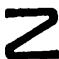
\includegraphics[keepaspectratio]{images/part003_6b42bd98.jpg}}

设 A 是 v 的环。若 v 是离散的，则 §3 第 6 节命题 8 表明 \(T_{v}\) 在 A 上诱导的拓扑是 m(A)-进拓扑。一般情形并非如此（习题 4）。

命题 2. 设 K 是一个未必交换的域，v 是 K 上一个非真的赋值，A 是 v 的环，m 是 v 的理想。赋以拓扑 \(\mathcal{T}_v\) 的 K 为局部紧的，当且仅当下列条件成立：

\begin{enumerate}
\def\labelenumi{(\roman{enumi})}
\item
  K 是完备的；
\item
  v 是离散的；
\item
  剩余域 \(\kappa(A)\) 是有限的。
\end{enumerate}

若是这样，则 A 是紧的。

设 K 是局部紧的。那么它是完备的（《一般拓扑学》第三章 § 3 第 3 节命题 4 的推论 1）；此外存在 0 的一个紧邻域，它包含某个邻域 \(\mathbf{V}_{\alpha}^{\prime}\) ，其中 \(\alpha\) 属于 \(v\) 的值群；换言之，存在 \(a \neq 0\) 在 \(\mathbf{K}^*\) 中，使得 A.a 是紧的，于是 \(\mathrm{A} = (\mathrm{A}.a)a^{-1}\) 是紧的。由于 A 的每个理想 \(\mathfrak{b} \neq (0)\) 都是开的，A/b 是紧的且离散的（《一般拓扑学》第三章 § 2 第 5 节命题 14），因而是有限的，特别地 \(\kappa(\mathrm{A}) = \mathrm{A}/\mathfrak{m}\) 是有限的。此外，对 \(y \neq 0\) （在 \(\mathfrak{m}\) 中），环 A/Ay 是有限的，故 A 中含 Ay 的理想只有有限多个，从而形如 \(v(x)\) 且满足

\[
0 <   v (x) \leqslant v (y)
\]

的元素组成的集合 P 是有限的；由于 \(v(\mathbf{K}^{*})\) 是全序的，P 有最小元素 \(\gamma\) 。于是对一切 \(x \in A\) （满足 \(v(x) > 0\) ），或者 \(v(x) > v(y) \geqslant \gamma\) ，或者 \(v(x) \leqslant v(y)\) 而按定义有 \(v(x) \geqslant \gamma\) ，所以 \(\gamma\) 是 \(v(\mathbf{K}^{*})\) 中 >0 的元素中最小的。由于 P 有限，存在最大整数 \(m \geqslant 0\) 使得 \(m_{\gamma} \in P\) ，于是 \(m\gamma \leqslant v(y) < (m + 1)\gamma.\) 由此得出 \(0 \leqslant v(y) - m\gamma < \gamma\) ，由 \(\gamma\) 的定义这蕴含 \(v(y) = m\gamma.\) 因此 \(v(\mathbf{K}^{*}) = \mathbf{Z}. \gamma\) ，赋值 \(v\) 是离散的。

反之，设条件 (i)、(ii)、(iii) 成立。可以只限于 v 是赋范的情形；设 u 是 v 的一个单值化元。那么 \(\kappa(\mathbf{A}) = \mathbf{A}/\mathbf{A}u\) ，因而 A/Au 是有限的。由于 \(x \mapsto xu^{n}\) 通过取商定义了加法群 A/Au 到 \(Au^{n}/Au^{n+1}\) 上的一个同构，故 \(A/Au^{j}\) 对一切 \(j \geqslant 0\) 是有限的。由于 A 在 K 中是闭的，它是完备的，因而同构于诸 \(A/Au^{j}\) 的逆极限（《一般拓扑学》第三章 §7 第 3 节命题 2），因此是紧的。既然 A 在 K 中是开的，由此可知 K 是局部紧的。

注. 注意在此证明中只需假设 A 是完备的。

我们将在 § 9 中看到，满足命题 2 中条件的域 K 有一个中心，它或者是 p-进域的有限代数扩张，或者是有限域上的形式幂级数域 \(\mathbf{F}_{q}((\mathbf{T}))\) ；此外 K 在其中心上是有限秩的。

\subsection{带赋值的域上的拓扑向量空间}

通篇设 K 是一个（未必交换的）域，v 是 K 上的一个赋值，G 是它的阶群。K 赋以拓扑 \(T_{v}\) 。

命题 3. 设 E 是 K 上的一个 Hausdorff 的、维数为 1 的左拓扑向量空间。假设 v 不是非真的。对 E 中一切 \(x_{0} \neq 0\) ，映射 \(a \mapsto ax_{0}\) 把 \(K_{s}\) 映到 E 上，是一个拓扑同构。

这个映射是连续的代数同构。只需证明它是双连续的。设 \(\alpha \in \mathbf{G}\) 。需要证明存在 E 中 0 的一个邻域 V，使得关系 \(ax_0 \in \mathbf{V}\) 蕴含 \(v(a) > \alpha\) 。设 \(a_0 \in \mathbf{K}^*\) 满足 \(v(a_0) = \alpha\) 。由于 E 是 Hausdorff 的，存在 E 中 0 的邻域 W 使得 \(a_0 x_0 \notin \mathbf{W}\) 。由于 \(v\) 不是非真的，存在 E 中 0 的邻域 W' 与 G 的元素 \(\beta\) ，使得关系 \(y \in \mathbf{W}'\) 与 \(v(a) \geqslant \beta\) 蕴含 \(ay \in \mathbf{W}\) 。设 \(a_1 \in \mathbf{K}^*\) 满足 \(v(a_1) = -\beta\) 。关系 \(ax_0 \in a_1^{-1} \mathbf{W}'\) 与 \(v(a) \leqslant \alpha\) 蕴含 \(a_1 ax_0 \in \mathbf{W}'\) 以及 \(v(a_0 a^{-1} a_1^{-1}) = \alpha + \beta - v(a) \geqslant \beta\) ，因而 \(a_0 x_0 = a_0 a^{-1} a_1^{-1}(a_1 ax_0) \in \mathbf{W}\) ，这是荒谬的；换言之，关系 \(ax_0 \in a_1^{-1} \mathbf{W}\) 蕴含 \(v(a) > \alpha\) 。

推论. 设 E 是 K 上的一个左拓扑向量空间，H 是 E 的一个闭超平面，D 是 E 的一个一维向量子空间且为 H 的代数余子空间。假设 v 不是非真的。那么 D 是 H 的拓扑余子空间。

考虑到命题 1 与命题 3，其证明与《拓扑向量空间》第一章 § 2 定理 1 的推论 2 相同。

命题 4. 假设 \(v\) 不是非真的且 \(K\) 是完备的。设 \(E\) 是 \(K\) 上的一个左拓扑向量空间，它是 Hausdorff 的且维数有限为 \(n\) 。对每个基 \((e_i)_{1 \leqslant i \leqslant n}\) （\(E\) 在 \(K\) 上的），映射 \((a_i) \mapsto \sum_{i=1}^{n} a_i e_i\) 由 \(K_s^n\) 到 \(E\) 上是拓扑向量空间同构。

考虑到命题 3 及其推论，其证明与《拓扑向量空间》第一章 § 2 定理 2 相同。

推论. 假设 v 不是非真的且 K 是完备的。设 E 是 K 上的一个 Hausdorff 拓扑向量空间，F 是 E 的一个有限维向量子空间。那么 F 是闭的。

F 是完备的。

\subsection{带赋值的域的完备化}

命题 5. 设 K 是一个未必交换的域，v 是 K 上的一个赋值，G 是赋以离散拓扑的群 \(v(\mathbf{K}^{*})\) 。

\begin{enumerate}
\def\labelenumi{(\alph{enumi})}
\item
  完备化环 \(\hat{\mathbf{K}}\) （即 \(\mathbf{K}\) 赋以 \(\mathcal{T}_v\) 后的完备化）是一个拓扑域。
\item
  映射 \(v: \mathbf{K}^* \to \mathbf{G}\) 可以唯一地延拓为连续映射 \(\hat{v}: \hat{\mathbf{K}}^* \to \mathbf{G}\) 。映射 \(\hat{v}\) （用 \(\hat{v}(0) = +\infty\) 加以延拓）是 \(\hat{\mathbf{K}}\) 上的一个赋值，且 \(\hat{v}(\hat{\mathbf{K}}^*) = v(\mathbf{K}^*)\) 。
\item
  \(\hat{\mathbf{K}}\) 上的拓扑是由赋值 \(\hat{v}\) 定义的拓扑。
\item
  对一切 \(\alpha \in \mathbf{G}\) ，设 \(\mathrm{V}_{\alpha}, \mathrm{V}_{\alpha}'\) 是 \(\mathbf{K}\) 的子群，由条件 \(v(x) > \alpha\) 、\(v(x) \geqslant \alpha\) 定义。那么 \(\overline{\mathrm{V}}_{\alpha}, \overline{\mathrm{V}}_{\alpha}'\) （\(\mathrm{V}_{\alpha}, \mathrm{V}_{\alpha}'\) 在 \(\hat{\mathbf{K}}\) 中的闭包）分别由条件 \(\hat{v}(x) > \alpha\) 、\(\hat{v}(x) \geqslant \alpha\) 定义。
\item
  \(\hat{v}\) 的环是 \(\hat{\mathbf{A}}\) ，即环 \(\mathbf{A}\) （\(v\) 的环）的完备化；\(\hat{v}\) 的理想是 \(\hat{\mathfrak{m}}\) ，即理想 \(\mathfrak{m}\) （\(v\) 的理想）的完备化。
\item
  \(\hat{\mathbf{A}} = \mathbf{A} + \hat{\mathfrak{m}}\) ；\(\hat{v}\) 的剩余域典范地等同于 \(v\) 的剩余域。
\end{enumerate}

为证明 (a) ，只需（《一般拓扑学》第三章 § 6 第 8 节命题 7）证明下述结论：设 \(\mathfrak{F}\) 是 \(\mathbf{K}^*\) 上（关于加法一致结构的）一个 Cauchy 滤子，0 不是它的触点；那么 \(\mathfrak{F}\) 在双射 \(x \mapsto x^{-1}\) 下的像是一个（关于加法一致结构的）Cauchy 滤子。因为 0 不是 \(\mathfrak{F}\) 的触点，故存在 \(\mathbf{M} \in \mathfrak{F}\) 与 \(\beta \in \mathbf{G}\) 使得 \(\beta\) 是 \(v(\mathbf{M})\) 的一个上界。设 \(\alpha \in \mathbf{G}\) 。若 \(\mathbf{M}'\) 是 \(\mathfrak{F}\) 的一个含于 \(\mathbf{M}\) 的元素，且 \(v(x - y) > \sup (\alpha + 2\beta, \beta)\) 对 \(x \in \mathbf{M}'\) 与 \(y \in \mathbf{M}'\) 成立，则 \(v(x^{-1} - y^{-1}) > \alpha\) 对 \(x \in \mathbf{M}'\) 与 \(y \in \mathbf{M}'\) 成立（第 1 节引理 1）。由此得 (a) 。

由第 1 节命题 1，\(v|K^*\) 是 \(K^*\) 到 \(G\) 的连续同态，因此可以唯一地延拓为连续同态 \(\hat{v}\) （由 \(K^*\) 到 \(G\) ）。关系式

\[
\hat {v} (x + y) \geqslant \inf (\hat {v} (x), \hat {v} (y))
\]

在 \(\mathbf{K}^*\) 中成立，因而由连续性在 \(\hat{\mathbf{K}}^*\) 中也成立。于是 \(\vartheta\) （用 \(\hat{\upsilon}(0) = +\infty\) 加以延拓）是 \(\hat{\mathbf{K}}\) 上的一个赋值，(b) 得证。

现在证明 (d) 。设 \(\alpha \in G\) ，\(x \in \overline{V}_{\alpha} - \{0\}\) 。当 \(y\) 在 \(V_{\alpha}\) 中充分接近 \(x\) 时，有 \(\hat{v}(x) = \hat{v}(y) = v(y)\) ，因而 \(\hat{v}(x) > \alpha\) 。反之，设 \(x \in \widehat{K}^*\) 满足 \(\hat{v}(x) > \alpha\) ；当 \(y\) 在 \(K^*\) 中充分接近 \(x\) 时，有 \(v(y) = \hat{v}(y) = \hat{v}(x)\) ，因此 \(y \in V_{\alpha}\) ，于是 \(x \in \overline{V}_{\alpha}\) 。这样，\(\overline{V}_{\alpha}\) 是由这样的 \(x \in \widehat{K}\) 组成的集合：\(\hat{v}(x) > \alpha\) 。对 \(V_{\alpha}'\) 论证类似。这就证明了 (d) 。

考虑到《一般拓扑学》第三章 § 3 第 4 节命题 7，断言 (c) 是 (d) 的推论。断言 (e) 是 (d) 的特例。最后设 \(x \in \hat{\mathbf{A}}\) ；存在 \(y \in \mathbf{A}\) 使得 \(\hat{v}(x - y) > 0\) ；于是 \(z = x - y \in \hat{\mathfrak{m}}\) ，因而 \(x = y + z \in \mathbf{A} + \hat{\mathfrak{m}}\) ；这样 \(\hat{\mathbf{A}} = \mathbf{A} + \hat{\mathfrak{m}}\) ，这证明了 (f) 。

注. 对一切 \(x \in \hat{\mathbf{K}}\) （不属于 \(\hat{\mathbf{A}}\) ），存在 \(x_0 \in \mathbf{K}\) 使得 \(\hat{v}(x - x_0) > 0\) ，\(\hat{v}(x) = \hat{v}(x_0) = v(x_0) < 0\) ；于是 \(x_0^{-1}x \in \hat{\mathbf{A}}\) ，且由于 \(x_0^{-1} \in \mathbf{A}\) ，可见若令 \(S = A - \{0\}\) ，就可以写成 \(\hat{\mathbf{K}} = S^{-1}\hat{\mathbf{A}}\) 。

\section{绝对值}

\subsection{关于绝对值的预备知识}

设 K 是一个域（交换或非交换）。回顾（《一般拓扑学》第九章 §3 第 2 节定义 2），K 上的绝对值是指 K 到 \(R_{+}\) 的满足下列公理的任一映射 f：

\((\mathrm{VA}_{\mathbf{I}})\) 关系 \(f(x) = 0\) 等价于 \(x = 0\) 。

\((\mathrm{VA}_{\mathrm{II}}) f(xy) = f(x)f(y)\) 对一切 \(x, y\) （在 \(\mathbf{K}\) 中）成立。

\((\mathrm{VA}_{\mathrm{III}}) f(x + y) \leqslant f(x) + f(y)\) 对一切 \(x, y\) （在 \(\mathbf{K}\) 中）成立。

由 \((\mathrm{VA}_{\mathbf{I}})\) 与 \((\mathrm{VA}_{\mathbf{II}})\) 可得 \(f(1) = 1, f(-1) = 1\) 以及

\[
f (x ^ {- 1}) = \frac {1}{f (x)}
\]

对 \(x \neq 0\) 成立。

对映射 \(f\) （由 \(\mathbf{K}\) 到 \(\mathbf{R}_{+}\) ）与实数 \(\mathbf{A} > 0\) ，用 \((\mathrm{U}_{\mathbf{A}})\) 表示关系

\[
f (x + y) \leqslant \mathrm{A}. \sup (f (x), f (y)) \quad \text {   for   all   } x, y \text {   in   } \mathrm{K}.
\]

我们用 \(\mathcal{V}(\mathbf{K})\) 表示由映射 \(f\) （从 \(\mathbf{K}\) 到 \(\mathbf{R}_{+}\) ）组成的集合，这些映射满足 \((\mathrm{VA}_{\mathbf{I}})\) 与 \((\mathrm{VA}_{\mathbf{II}})\) ，且存在 \(\mathbf{A} > 0\) （依赖于 \(f\) ）使 \((\mathbf{U}_{\mathbf{A}})\) 成立。

注意，若 \(f \in \mathcal{V}(\mathbf{K})\) ，则把 \(x = 1, y = 0\) 代入 \((\mathrm{U}_{\mathbf{A}})\) ，

\[
1 = f (1) \leqslant A. \sup (f (1), f (0)) = A.
\]

命题 1. 映射 \(f\) （从 \(\mathbf{K}\) 到 \(\mathbf{R}_+\) ）满足 \((\mathrm{VA}_{\mathbf{I}})\) 与 \((\mathrm{VA}_{\mathbf{II}})\) 而属于 \(\mathcal{V}(\mathbf{K})\) ，当且仅当 \(f(1 + x)\) 在由这样的 \(x \in \mathbf{K}\) （满足 \(f(x) \leqslant 1\) ）组成的集合上有界。

若 \(f\) 满足 \((\mathrm{U}_{\mathbf{A}})\) ，则 \(f(1 + x) \leqslant \mathbf{A}\) 当 \(f(x) \leqslant 1\) 时成立。反之，设 \(f(x + 1) \leqslant \mathbf{A}\) 对这样的 \(x \in \mathbf{K}\) （满足 \(f(x) \leqslant 1\) ）成立（这蕴含 \(\mathbf{A} \geqslant f(1) = 1\) ）；那么，若 \(x = 0\) 或 \(y = 0\) ，条件 \((\mathrm{U}_{\mathbf{A}})\) 成立；另一方面，若 \(x \neq 0\) 且 \(y \neq 0\) ，不妨设 \(f(y) \leqslant f(x)\) ，于是由 \((\mathrm{VA}_{\mathrm{II}}), f(yx^{-1}) \leqslant 1\) ，因此 \(f(1 + yx^{-1}) \leqslant \mathbf{A}\) ，由 \((\mathrm{VA}_{\mathrm{II}}), f(x + y)f(x)^{-1} \leqslant \mathbf{A}\) ；从而

\[
f (x + y) \leqslant A f (x) \leqslant A. \sup (f (x), f (y)).
\]

若 \(f\) 是 \(\mathbf{K}\) 上的绝对值，则 \(f(n,1) \leqslant n\) 对整数 \(n > 0\) 从 \((\mathrm{VA}_{\mathrm{III}})\) 出发用归纳法可得；反之：

命题 2. 设 \(f\) 是 \(\mathbf{K}\) 到 \(\mathbf{R}_+\) 的一个映射，且属于 \(\mathcal{V}(\mathbf{K})\) ；若存在 \(\mathbf{C} > 0\) 使得 \(f(n,1) \leqslant \mathbf{C}.n\) 对每个整数 \(n > 0\) 成立，则 \(f\) 是 \(\mathbf{K}\) 上的绝对值。

对 r > 0 作归纳，由 \((\mathbf{U}_{\mathbf{A}})\) 推出关系

\[
f (x _ {1} + x _ {2} + \dots + x _ {2 ^ {r}}) \leqslant A ^ {r} \sup _ {1 \leqslant i \leqslant 2 ^ {r}} f (x _ {i})\tag{1}
\]

对每个族 \((x_{i})\) ——由 \(2^{r}\) 个 \(\mathbf{K}\) 的元素组成——成立。令 \(n = 2^{r} - 1\) ；对一切 \(x \in \mathbf{K}\) ，由 (1) 推出

\[
(f (1 + x)) ^ {n} = f ((1 + x) ^ {n}) = f \left(\sum_ {i = 0} ^ {n} \binom {n} {i} x ^ {i}\right) \leqslant A ^ {r} \sup \left(f \left(\binom {n} {i}\right) (f (x)) ^ {i}\right)
\]

\[
\leqslant \mathrm{CA} ^ {r} \sum_ {i = 0} ^ {n} \binom {n} {i} (f (x)) ^ {i} = \mathrm{CA} ^ {r} (1 + f (x)) ^ {n}
\]

因为 \(f\left(\binom{n}{i}\right) \leqslant C\binom{n}{i}\) ；因此

\[
f (1 + x) \leqslant \mathrm{C} ^ {1 / n} \mathrm{A} ^ {r / n} (1 + f (x)).
\]

令 r 趋于 \(+\infty\) ，得到 \(f(1+x)\leqslant1+f(x)\) 对一切 \(x\in K\) 成立；把 x 换成 \(xy^{-1}\) （其中 \(y\neq0\) ）应用这个不等式，并注意到 \((\mathrm{VA}_{\mathrm{II}})\) ，就得到关系 \((\mathrm{VA}_{\mathrm{III}})\) ，这证明了命题。

推论 1. 由 K 到 \(R_{+}\) 的映射 f 是绝对值，当且仅当它满足条件 (VA \(_{I}\) )、(VA \(_{II}\) ) 与 (U \(_{2}\) )。

这是必要的，因为 \((\mathrm{VA}_{\mathrm{II}})\) 蕴含

\[
f (x + y) \leqslant f (x) + f (y) \leqslant 2 \sup (f (x), f (y)).
\]

反之，设 \(f\) 满足 \((\mathrm{VA}_{\mathrm{I}}), (\mathrm{VA}_{\mathrm{II}})\) 与 \((\mathrm{U}_2)\) ；对每个整数 \(n > 0\) ，设 \(r\) 是使 \(2^r \geqslant n\) 的最小整数；若在 (1) 中把 A 换成 2，把 \(x_i\) 中指标 \(i \leqslant n\) 的换成 1，把 \(x_i\) 中指标 \(i > n\) 的换成 0，就得到

\[
f (n. 1) \leqslant 2 ^ {r} <   2 n;
\]

于是可以取 \(\mathbf{C} = 2\) 应用命题 2，因而 \(f\) 是绝对值。

推论 2. 映射 \(f\) （由 \(\mathbf{K}\) 到 \(\mathbf{R}_+\) ）属于 \(\mathcal{V}(\mathbf{K})\) ，当且仅当它形如 \(g^t\) ，其中 \(t > 0\) 且 \(g\) 是 \(\mathbf{K}\) 上的绝对值。

说 \(f\) 满足 \((\mathbf{U}_{\mathbf{A}})\) 等价于说 \(f^s\) 满足 \((\mathbf{U}_{\mathbf{A}^s})\) ；由于存在 \(s > 0\) 使 \(\mathbf{A}^s \leqslant 2\) ，推论 1 表明对这样的值，\(s, f^s\) 是绝对值。

\subsection{超度量绝对值}

由 K 到 \(R_{+}\) 的映射 f 若满足条件 ( \(VA_{I}\) )、( \(VA_{II}\) ) 与 ( \(U_{1}\) ) （这显然蕴含 f 是绝对值），则称为超度量绝对值。

命题 3. 设 \(f\) 是由 \(\mathbf{K}\) 到 \(\mathbf{R}_+\) 的映射。下列性质等价：

\begin{enumerate}
\def\labelenumi{(\alph{enumi})}
\item
  \(f\) 是超度量绝对值。
\item
  存在一个赋值 \(v\) （在 \(\mathbf{K}\) 上取值于 \(\mathbf{R}\) ）以及实数 \(a\) ，使得 \(0 < a < 1\) 且 \(f = a^v\) 。
\item
  \(f\) 属于 \(\mathcal{V}(\mathbf{K})\) ，且 \(f(n,1) \leqslant 1\) 对每个整数 \(n > 0\) 成立。
\item
  对一切 \(s > 0, f^s\) 是绝对值。
\end{enumerate}

对每个实数 \(c\) （满足 \(0 < c < 1\) ），映射 \(t \mapsto c^t\) 是有序群 \(\mathbf{R}\) （带与通常序相反的序）到有序群 \(\mathbf{R}_+^*\) 上的同构；这表明 (a) 与 (b) 等价。显然 (a) 蕴含 (c)；(c) 蕴含 (d)，因为由 (c) 推出

\[
(f (n. 1)) ^ {s} \leqslant 1 \leqslant n
\]

对每个整数 \(n > 0\) 成立，而第 1 节命题 2 表明 \(f^s\) 是绝对值。最后 (d) 蕴含 (a)：因为若 \(f^s\) 是绝对值，它就满足 \((\mathbf{U}_2)\) ，因而 \(f\) 满足 \((\mathbf{U}_{2^{1 / s}})\) 对一切 \(s > 0\) 成立，因此它也满足 \((\mathbf{U}_1)\) ，令 \(s\) 趋于 \(+\infty\) 。

推论. 若 K 是特征 p > 0 的（未必交换的）域，则 \(\mathcal{V}(\mathbf{K})\) 上的每个函数都是超度量绝对值。

每个非零元素 \(z = n.1\) （ \(n\) 为整数 \(>0\) ）都属于素子域 \(\mathbf{F}_p\) （\(K\) 的），因而满足关系 \(z^{p-1} = 1\) ，这蕴含 \(f(z) = 1\) ，于是可以应用命题 3 (c)。

给定实数 \(c\) （满足 \(0 < c < 1\) ），公式

\[
f (x) = c ^ {v (x)}, \quad v (x) = \log_ {c} f (x)
\]

就在 K 上的超度量绝对值与 K 上取实值的赋值之间建立了一一对应。非真赋值对应于非真绝对值（《一般拓扑学》第九章 § 3 第 2 节）。设 \(v_{1}, v_{2}\) 是 K 上两个取实值的赋值，\(f_{1}, f_{2}\) 是相应的绝对值；\(v_{1}\) 与 \(v_{2}\) 等价，当且仅当 \(f_{1}\) 与 \(f_{2}\) 等价：因为说 \(v_{1}\) 与 \(v_{2}\) 等价，相当于说关系 \(v_{1}(x) \geqslant 0\) 与 \(v_{2}(x) \geqslant 0\) 等价，或者再说关系 \(f_{1}(x) \leqslant 1\) 与 \(f_{2}(x) \leqslant 1\) 等价；因此只需应用《一般拓扑学》第九章 §3 第 2 节命题 5。此外（同前），由 \(f_{1}\) 与 \(f_{2}\) 在 K 上定义的拓扑相同，当且仅当 \(f_{1}\) 与 \(f_{2}\) 等价。

\subsection{Q 上的绝对值}

命题 4. 设 \(f\) 是 \(\mathbf{Q}\) 到 \(\mathbf{R}_+\) 的一个映射，且属于 \(\mathcal{V}(\mathbf{Q})\) 。那么：

\begin{enumerate}
\def\labelenumi{(\roman{enumi})}
\item
  或者 \(f\) 是 \(\mathbf{Q}\) 上的非真绝对值。
\item
  或者存在实数 \(a\) 与素数 \(p\) ，使得 \(0 < a < 1\) 且 \(f = a^{v_p}\) ，其中 \(v_p\) 是 \(p\) -进赋值。
\item
  或者存在 \(s > 0\) ，使得 \(f(x) = |x|^s\) 对一切 \(x \in \mathbf{Q}\) 成立。
\end{enumerate}

在情形 (iii) 中，\(f\) 是 \(\mathbf{Q}\) 上的绝对值，当且仅当 \(0 < s \leqslant 1\) 。

首先设 \(f(n) \leqslant 1\) 对每个整数 \(n > 0\) 成立。由第 2 节命题 3，存在实数 \(b\) 与赋值 \(v\) （\(\mathbf{Q}\) 上的），使得 \(0 < b < 1\) 且 \(f = b^v\) 。而我们知道（§ 3 第 4 节例 4），\(\mathbf{Q}\) 上（在等价的意义下）仅有的赋值是非真赋值与诸 \(p\) -进赋值 \(v_p\) ；因此或者出现情形 (i)，或者出现情形 (ii)。

从现在起设存在整数 \(h > 0\) 使得 \(f(h) > 1\) ；由第 1 节命题 2 的推论 2，存在数 \(\rho > 0\) 使得 \(f^{\rho}\) 是绝对值；记

\[
g (x) = \rho \log (f (x)) / \log | x |
\]

对每个有理数 \(x \neq 0\) 成立。设 \(a, b\) 是两个 \(\geqslant 2\) 的整数；对每个整数 \(n \geqslant 2\) ，用 \(q(n)\) 表示 \(n\) . log \(a / \log b\) 的整数部分，换句话说即最小的整数 \(m\) ，使 \(a^n < b^{m+1}\) ；于是 \(a^n\) 以 \(b\) 为底的展开为

\[
a ^ {n} = c _ {0} + c _ {1} b + \dots + c _ {q (n)} b ^ {q (n)}\tag{2}
\]

其中 \(0 \leqslant c_{i} < b\) 对 \(0 \leqslant i \leqslant q(n)\) 成立。由于 \(f^{\rho}\) 是绝对值，\(f^{\rho}(c_{i}) \leqslant c_{i} \leqslant b\) ，于是由 (2) 推出

\[
\begin{array}{r l} (f (a)) ^ {n \rho} = (f (a ^ {n})) ^ {\rho} & \leqslant b (1 + (f (b)) ^ {\rho} + \dots + (f (b)) ^ {\rho q (n)}) \\ & \leqslant b (q (n) + 1) (\sup (1, (f (b)) ^ {\rho})) ^ {q (n)}. \end{array}
\]

对这个不等式的两边取对数并除以 \(n.\log a\) ，得到

\[
g (a) \leqslant \frac {\log b}{n . \log a} + \frac {\log (q (n) + 1)}{q (n)} \cdot \frac {q (n)}{n . \log a} + \frac {\sup (0 , \rho \log f (b))}{\log a} \cdot \frac {q (n)}{n}.\tag{3}
\]

现在注意，当 \(n\) 趋于 \(+\infty\) 时，\(q(n) / n\) 趋于 \(\log a / \log b\) ；因此 \(q(n)\) 趋于 \(+\infty\) 且

\[
\log (q (n) + 1) / q (n)
\]

趋于 0（《实变函数》第三章 § 2 第 1 节）。在 (3) 中取极限，得到

\[
g (a) \leqslant \frac {\sup (0 , \rho \log f (b))}{\log b} = \sup (0, g (b)).\tag{4}
\]

但 \(f(h) > 1\) ，于是 \(g(h) > 0\) ；若在 (4) 中把 \(a\) 换成 \(h\) ，就得到 \(\sup(0, g(b)) > 0\) ，从而

\[
\sup (0, g (b)) = g (b).
\]

于是，对任意至少等于 2 的整数 \(a\) 、\(b\) ，有 \(g(a) \leqslant g(b)\) ，从而 \(g(a) = g(b)\) （交换 \(a\) 与 \(b\) 的角色）。换言之，存在常数 \(\lambda\) 使得 \(g(a) = \lambda\) 对每个整数 \(a \geqslant 2\) 成立；若记 \(s = \lambda / \rho\) ，则 \(f(a) = |a|^s\) 对每个整数 \(a \geqslant 2\) 成立。由于 \(f(xy) = f(x)f(y)\) 且 \(f(-x) = f(x) = |x|^s\) 对一切 \(x \in \mathbf{Q}\) 。最后，若 \(0 < s \leqslant 1\) ，我们知道 \(x \mapsto |x|^s\) 是绝对值（《一般拓扑学》第九章 §3 第 2 节）；反之，若 \(s\) 使 \(x \mapsto |x|^s\) 是 \(\mathbf{Q}\) 上的绝对值，则 \((1 + 1)^s \leqslant 1^s + 1^s\) ，即 \(2^s \leqslant 2\) ，于是 \(s \leqslant 1\) 。

\subsection{具有非超度量绝对值的域的结构}

定理 1 （Gelfand-Mazur）. 设 \(\mathbf{K}\) 是域 \(\mathbf{R}\) 上的一个代数，具有下面两条性质：

\begin{enumerate}
\def\labelenumi{(\arabic{enumi})}
\item
  K 是一个（未必交换的）域。
\item
  K 上存在与 K 上的代数结构相容的范数 \(x \mapsto \| x \|\) （《一般拓扑学》第九章 § 3 第 7 节定义 9）。
\end{enumerate}

那么代数 \(\mathbf{K}\) 同构于代数 \(\mathbf{R},\mathbf{C}\) 或 \(\mathbf{H}\) 之一。

回顾（同前），总可以假定对 K 中一切 x,y 有 \(\|xy\|\leqslant\|x\|. \|y\|\) 。我们将给 K 以由该范数定义的（与代数结构相容的）拓扑。

\textbf{(A) 第一种情形：\(\mathbf{K}\) 是交换的且存在 \(j\in \mathbf{K}\) 使得 \(j^2 = -1\)}\par

那么存在一个同构 \(\sigma\) ，它把域 \(\mathbf{C}\) 映到 \(\mathbf{K}\) 的一个子域上，使得 \(\sigma(\xi + i\eta) = \xi \cdot 1 + \eta \cdot j\) 对 \(\xi, \eta\) （在 \(\mathbf{R}\) 中）成立。我们将用反证法证明 \(\mathbf{K} = \sigma(\mathbf{C})\) 。于是设存在 \(x \in \mathbf{K} - \sigma(\mathbf{C})\) ；那么对一切 \(z \in \mathbf{C}, x - \sigma(z)\) 在 \(\mathbf{K}\) 中可逆；记 \(\mathrm{F}(z) = (x - \sigma(z))^{-1}\) ；由于 \(\sigma\) 连续且取逆在 \(\mathbf{K}\) 上连续（《一般拓扑学》第九章 §3 第 7 节命题 13 应用于 \(\mathbf{K}\) 的完备化代数），\(\mathbf{F}\) 是 \(\mathbf{C}\) 到 \(\mathbf{K}\) 的连续映射。此外，对 \(z \neq 0\) 可以写成

\[
\mathrm{F} (z) = (\sigma (z)) ^ {- 1} (x (\sigma (z)) ^ {- 1} - 1) ^ {- 1}.
\]

但由 \((\sigma(z))^{-1} = \sigma(z^{-1})\) 当 \(z\) 在 \(\mathbf{C}\) 中趋于无穷时趋于 0，可见 \(\mathbf{F}(z)\) 趋于 0；换言之，\(z \mapsto \| \mathbf{F}(z) \|\) 是连续的实值函数，\(\geqslant 0\) （在 \(\mathbf{C}\) 上），在无穷远点趋于 0，因而可以看作紧空间 \(\tilde{\mathbf{C}}\) （由 \(\mathbf{C}\) 添加一个无穷远点而得）上的连续函数。于是 \(\alpha\) （\(\| \mathbf{F} \|\) 在 \(\mathbf{C}\) 上的上确界）有限且 \(>0\) ，且集合 \(\mathrm{P}\) ——由复数 \(z\) （满足 \(\| \mathrm{F}(z) \| = \alpha\) ）组成的——是闭的且非空（《一般拓扑学》第四章 §6 第 1 节定理 1）。

设 \(z \in \mathbf{P}\) ；记 \(y = x - \sigma(z)\) ，并设 \(t\) 是一个复数 \(\neq 0\) 使得 \(\| \sigma(t) \| < \alpha^{-1}\) ，于是 \(\| \sigma(t).y^{-1} \| < 1\) （由 \(\alpha\) 的定义）。因此，序列 \((\sigma(t)y^{-1})^n\) 与序列 \(n(\sigma(t)y^{-1})^n\) 在 \(K\) 中都趋于 0（当 \(n\) 趋于 \(+\infty\) 时），因为它们在 \(R\) 中的相应范数序列如此。另一方面注意，对每个多项式 \(\mathbf{H}(\mathbf{T}) = \prod_{k=1}^{p} (\mathbf{T} - \sigma(c_k))\) （其中诸 \(c_k\) 是互异的复数），在有理函数域 \(\mathbf{K}(\mathbf{T})\) 中

\[
\frac {\mathrm{H} ^ {\prime} (\mathrm{T})}{\mathrm{H} (\mathrm{T})} = \sum_ {k = 1} ^ {p} \frac {1}{\mathrm{T} - \sigma (c _ {k})}.\tag{5}
\]

把这个公式应用于多项式

\[
\mathrm{H} (\mathrm{T}) = \mathrm{T} ^ {n} - (\sigma (t)) ^ {n} = \prod_ {k = 0} ^ {n - 1} \left(\mathrm{T} - \sigma \left(\omega_ {n} ^ {k} t\right)\right),
\]

其中 \(\omega_{n}=\exp(2\pi i/n)\) ，并把 T 换成元素 \(y\in K\) ，它与所有 \(\sigma(\omega_{n}^{k}t)\) 都不同。由此（在交换域 K 中）得到

\[
\frac {n y ^ {n - 1}}{y ^ {n} - (\sigma (t)) ^ {n}} = \frac {1}{y - \sigma (t)} + \sum_ {k = 1} ^ {n - 1} \frac {1}{y - \sigma \left(\omega_ {n} ^ {k} t\right)}.\tag{6}
\]

考虑到 F 与 y 的定义，得到

\[
\begin{array}{r l} \mathrm{F} (z + t) + \sum_ {k = 1} ^ {n - 1} \mathrm{F} (z + \omega_ {n} ^ {k} t) - n \mathrm{F} (z) & \\ = \frac {n y ^ {n - 1}}{y ^ {n} - (\sigma (t)) ^ {n}} - \frac {n}{y} = \frac {1}{y} \cdot \frac {n (\sigma (t) y ^ {- 1}) ^ {n}}{1 - (\sigma (t) y ^ {- 1}) ^ {n}}. \end{array}\tag{7}
\]

但由 t 的选取及上面的注记，(7) 中的最后一个表达式当 n 趋于 \(+\infty\) 时趋于 0；从而

\[
\| \mathrm{F} (z + t) \| = \lim _ {n \to + \infty} \| n \mathrm{F} (z) - \sum_ {k = 1} ^ {n - 1} \mathrm{F} (z + \omega_ {n} ^ {k} t) \|.\tag{8}
\]

现在，\(\| \mathrm{F}(z)\| = \alpha\) 且 \(\| \mathrm{F}(z + \omega_n^kt)\| \leqslant \alpha\) （由 \(\alpha\) 的定义），于是

\[
\left\| n \mathrm{F} (z) - \sum_ {k = 1} ^ {n - 1} \mathrm{F} (z + \omega_ {n} ^ {k} t) \right\| \geqslant
\]

\[
n \| \mathrm{F} (z) \| - \sum_ {k = 1} ^ {n - 1} \| \mathrm{F} (z + \omega_ {n} ^ {k} t) \| \geqslant n \alpha - (n - 1) \alpha = \alpha .
\]

因此由 (8)，令 \(n\) 趋于 \(+\infty\) ，得 \(\| \mathbf{F}(z + t) \| \geqslant \alpha\) ，再由 \(\alpha\) 的定义，这蕴含

\[
\| \mathrm{F} (z + t) \| = \alpha ,
\]

换言之 \(z + t \in P\) 。这证明集合 P 在 C 中是开的；由于它又是闭的且非空，而 C 是连通的，故 P = C ，于是 \(\|F\|\) 在 C 上是常数；由于这个函数在无穷远点趋于 0，在 C 中 \(\|F(z)\| = 0\) ，特别地 \(\|F(0)\| = \|x^{-1}\| = 0\) ，这是荒谬的。

\textbf{(B) 第二种情形；\(\mathbf{K}\) 是交换的且 \(-1\) 不是 \(\mathbf{K}\) 中元素的平方}\par

设 L 是由 K 添加 \(T^{2} + 1\) 的一个根 j 所得的交换域；L 是 K 上的向量空间，以 \((1, j)\) 为基，且 L 显然是 R 上的代数。显然，函数 \(x + yj \to \|x\| + \|y\|\) 是 L 上与其 R 上向量空间结构相容的范数；另一方面，对 L 中的 \(z = x + yj\) 、\(z' = x' + y'j\) ，

\[
\begin{array}{r l} \| z z ^ {\prime} \| & = \| x x ^ {\prime} - y y ^ {\prime} \| + \| x y ^ {\prime} + x ^ {\prime} y \| \leqslant \| x x ^ {\prime} \| + \| y y ^ {\prime} \| + \| x y ^ {\prime} \| + \| x ^ {\prime} y \| \\ & \leqslant \| x \| \cdot \| x ^ {\prime} \| + \| y \| \cdot \| y ^ {\prime} \| + \| x \| \cdot \| y ^ {\prime} \| + \| x ^ {\prime} \| \cdot \| y \| \\ & = (\| x \| + \| y \|) (\| x ^ {\prime} \| + \| y ^ {\prime} \|) = \| z \| \cdot \| z ^ {\prime} \|. \end{array}
\]

这样定义的范数因而与 L 上的 R-代数结构相容。由情形 (A)，L 是同构于 C 的 R-代数；而 C 的异于 C 的子 R-代数只有 R ，故 K 同构于 R 。

\textbf{(C) 第三种情形：K 非交换}\par

设 Z 是 K 的中心，x 是 K 中不属于 Z 的元素；K 的子域 \(Z(x)\) 是交换的，且由 K 上的范数诱导的范数与 \(Z(x)\) 上的 R-代数结构相容；由于 \(Z \neq Z(x)\) ，且由 (A) 与 (B)，Z 与 \(Z(x)\) 是同构于 R 或 C 的 R-代数，Z 必然同构于 R 而 \(Z(x)\) 同构于 C。于是对一切 \(x \in K\) ，\(Z(x)\) 在 Z 上的秩 \(\leqslant 2\) 。现在我们有下面的引理：

引理 1. 设 D 是以 L 为中心的域，使得对一切 \(x \in \mathbf{D}\) ，\(\mathbf{L}(x)\) 是 L 的次数 \(\leqslant m\) 的扩张。那么 D 在 L 上的秩 \(\leqslant m^2\) 。

显然可以只限于 \(D \neq L\) 的情形。那么 D 中存在 L 的一个次数 >1 的有限可分代数交换扩张 E （《代数》第八章 § 10 第 3 节引理 1）；由于对 E 中某个适当的 x 有 \(E = L(x)\) （《代数》第五章 § 7 第 7 节命题 12 及第七章 § 5 第 7 节），由假设 \([E: L] \leqslant m\) 。设取可分扩张 E 使 \([E: L]\) 有限且尽可能大，并考虑 E 在 D 中的中心化子 \(E' \supset E\) ，它是一个以 E 为中心的域，使得

\[
[ \mathbf {D} \colon \mathbf {E} ^ {\prime} ] = [ \mathbf {E} \colon \mathbf {L} ] \leqslant m
\]

（《代数》第八章 § 10 第 2 节定理 2）。若 \(\mathbf{E} \neq \mathbf{E}'\) ，则 \(\mathbf{E}'\) 中会存在一个有限可分代数扩张 \(\mathbf{F}\) （\(\mathbf{E}\) 的扩张），次数 \(>1\) （《代数》第八章 § 10 第 3 节引理 1）；于是 \(\mathbf{F}\) 会是 \(\mathbf{L}\) 的次数 \(>[\mathrm{E:L}]\) 的有限可分代数扩张（《代数》第五章 § 7 第 4 节命题 7），这与 \(\mathbf{E}\) 的定义矛盾；因此 \(\mathbf{E}' = \mathbf{E}\) ，从而 \([\mathrm{D:L}] = [\mathrm{D:E}][\mathrm{E:L}] \leqslant m^2\) 。

把这条引理以 m = 2 应用于 K，可见 K 是 R 的有限秩非交换扩张域，因而同构于四元数体 H （《代数》第八章 § 11 第 2 节定理 2）。

注 (1) 在讨论赋范代数的那一章中，我们将给出 Gelfand-Mazur 定理的一个较短的证明，它对 R 上每个 Hausdorff 局部凸拓扑代数 K 都成立，其原理如下：归结为（如在情形 (B) 与 (C) 中那样）K 是 C 上交换代数的情形；若 \(x \in K - C.1\) ，我们如上考虑 C 到 K 的映射 \(z \mapsto (x - z.1)^{-1}\) ，它在 C 上连续且可微。对每个元素 \(x'\) （属于局部凸空间 K 的对偶 \(K'\) ），\(z \mapsto \langle(x - z.1)^{-1}, x' \rangle\) 是 C 上的有界整函数，因而由 Liouville 定理是常数，于是如定理 1 的证明中 (A) 部分那样，可以断定这必然蕴含 \(\langle(x - z.1)^{-1}, x' \rangle = 0\) 对一切 \(z \in C\) 与一切 \(x' \in K'\) ；Hahn-Banach 定理表明这个结论是荒谬的，因为 \((x - z.1)^{-1} \neq 0\) 。注意，定理 1 证明中 (A) 部分的论证与上面的论证只是表面不同，因为这个论证只是用来证明解析函数最大模原理的论证的一个特例，对单位根求和并取极限等价于沿中心为 0 的圆计算积分 \(\int_{\gamma} \frac{F(z + t) dt}{t}\) ，而这里由于函数 F 的特殊形式，避免了使用 Cauchy 公式。

定理 2 （Ostrowski）. 设 K 是一个（未必交换的）域，f 是 \(\mathcal{V}(\mathbf{K})\) 中一个不是超度量绝对值的元素。那么存在唯一的实数 s > 0 以及 K 到域 R 、 C 或 H 之一的一个处处稠密子域上的同构 j ，使得 \(f(x) = |j(x)|^{s}\) 对一切 \(x \in K (*)\) 成立。f 是 K 上的绝对值，当且仅当 \(s \leqslant 1\) 。

由第 2 节命题 3 的推论，K 的特征为 0，因而是 Q 上的代数；对一切 \(x \in Q\) 记 \(h(x) = f(x.1)\) ；显然 \(h \in \mathcal{V}(\mathbf{Q})\) ，因此可以应用第 3 节命题 4；该命题陈述中的情形 (i) 与 (ii) 都不能出现，因为那将蕴含 \(f(n.1) \leqslant 1\) 对每个整数 n > 0 成立，从而由第 2 节命题 3，f 是超度量绝对值。于是存在实数 \(s > 0\) 使得 \(h(x) = |x|^s\) 对一切 \(x \in \mathbf{Q}\) 成立，即 \(f(x,1) = |x|^s\) ；记 \(g = f^{1 / s}\) 。那么 \(g \in \mathcal{V}(\mathbf{K})\) 且 \(g(n,1) = n\) 对每个整数 \(n\) 成立；因此第 1 节命题 2 表明 \(g\) 是 \(\mathbf{K}\) 上的绝对值。

对 \(x \in \mathbf{Q}\) 与 \(y \in \mathbf{K}\) ，有 \(g(xy) = |x|g(y)\) ，因而 \(g\) 是 \(\mathbf{K}\) 上与其 \(\mathbf{Q}\) -代数结构相容的范数（\(\mathbf{Q}\) 上取通常绝对值）。于是完备化 \(\hat{\mathbf{K}}\) （即 \(\mathbf{K}\) 的完备化）是 \(\hat{\mathbf{Q}} = \mathbf{R}\) 上的赋范代数（《一般拓扑学》第九章 § 3 第 7 节）；设 \(\hat{g}\) 是 \(\hat{\mathbf{K}}\) 上作为 \(g\) 的连续延拓的范数。由于 \(g\) 是 \(\mathbf{K}\) 上的绝对值，\(\hat{\mathbf{K}}\) 是域且 \(\hat{g}\) 是 \(\hat{\mathbf{K}}\) 上的绝对值（《一般拓扑学》第九章 § 3 第 3 节命题 6）。由定理 1，存在一个 \(\mathbf{R}\) -代数同构 \(j\) ，它把 \(\hat{\mathbf{K}}\) 映到域 \(\mathbf{R}\) 、\(\mathbf{C}\) 或 \(\mathbf{H}\) 之一上，于是 \(g'(x) = |j(x)|\) 是 \(\hat{\mathbf{K}}\) 上的绝对值；由于 \(\hat{\mathbf{K}}\) 在 \(\mathbf{R}\) 上有限维，且 \(g'\) 与 \(\hat{g}\) 在子域 \(\mathbf{R}\) . 1 （\(\hat{\mathbf{K}}\) 的）上一致，由下面的引理得 \(g' = \hat{g}\) ：

引理 2. 设 L 是一个（未必交换的）域，K 是 L 的子域，使得 L 是 K 上有限维左向量空间。设 g 是 L 上的绝对值，f 是它在 K 上的限制。若 K 关于 f 是完备的且非离散的，则 L 关于 g 是完备的；若进一步 \(g'\) 是 L 上另一个在 K 上有同一限制 f 的绝对值，则 \(g' = g\) 。

由于由 g 定义的拓扑是 Hausdorff 的且与 L 上的左向量 K-空间结构相容，第一个断言由《拓扑向量空间》第一章 § 2 第 3 节定理 2 得出。此外，由 g 与 \(g'\) 在 L 上定义的拓扑相同（同前）；因此存在实数 s > 0 使得 \(g' = g^{s}\) （《一般拓扑学》第九章 § 3 第 2 节命题 5）。设 x 是 K 中使 \(f(x) \neq 1\) 的元素；方程 \(g'(x) = g(x)\) 表明 s = 1 。

回到定理 2 的证明，可见若 \(j\) 表示 \(\hat{j}\) 在 \(\mathbf{K}, j\) 上的限制，则它是 \(\mathbf{K}\) 到 \(\mathbf{R}\) 、\(\mathbf{C}\) 或 \(\mathbf{H}\) 的一个处处稠密子域上的同构，且 \(g(x) = |j(x)|\) 对 \(x \in \mathbf{K}\) 成立，从而 \(f(x) = |j(x)|^s\) 。

最后注意，若 \(f\) 是 \(\mathbf{K}\) 上的绝对值，则 \(h\) 是 \(\mathbf{Q}\) 上的绝对值，且由第 3 节命题 4 有 \(s \leqslant 1\) ；反之，若 \(s \leqslant 1\) ，则 \(f = g^s\) 是 \(\mathbf{K}\) 上的绝对值，因为 \(g\) 是绝对值（《一般拓扑学》第九章 § 3 第 2 节）；这就证明了陈述中的最后一个断言。

\textbf{注}\par

\begin{enumerate}
\def\labelenumi{(\arabic{enumi})}
\setcounter{enumi}{1}
\item
  若 K 是域又是 R 上的赋范代数，其范数未必是 K 上的绝对值；例如，\(\xi + i\eta \to |\xi| + |\eta|\) 是 C 上与其 R-代数结构相容的范数。
\item
  定理 1 情形 (C) 的一个不使用《代数》第八章一般结果的证明，见习题 2。
\end{enumerate}

\section{逼近定理}

\subsection{有限个赋值环的交}

命题 1. 设 K 是域，\((\mathbf{A}_{i})_{1 \leqslant i \leqslant n}\) 是 K 的赋值环的有限族，\(B = \bigcap_{i=1}^{n} A_{i}\) 。记 \(p_{i} = B \cap m(A_{i})\) 。那么对一切 i 有 \(A_{i} = B_{p_{i}}\) ，且 B 的分式域是 K。

显然 \(B_{p_t} \subset A_t\) 。为证明相反的包含关系，我们需要下面的引理： 引理 1. 设 \(v_i (1 \leqslant i \leqslant n)\) 是域 \(K\) 上的赋值，\(x \in K^*\) 。那么存在一个形如下式的多项式 \(f(X)\)

\[
\begin{array}{l} (1) f (\mathbf {X}) = 1 + n _ {1} \mathbf {X} + \dots + n _ {k - 1} \mathbf {X} ^ {k - 1} + \mathbf {X} ^ {k} \\ \quad (k \geqslant 2, n _ {j} \in \mathbf {Z} for 1 \leqslant j \leqslant k - 1) \end{array}
\]

使得 \(f(x) \neq 0\) ，且元素 \(z = f(x)^{-1}\) 对 \(1 \leqslant i \leqslant n\) 具有下列性质：

\[
\begin{array}{l l} v _ {i} (z) = 0 & \text { if } \quad v _ {i} (x) \geqslant 0 \\ v _ {i} (z) + v _ {i} (x) > 0 & \text { if } \quad v _ {i} (x) <   0. \end{array}
\]

暂且承认这条引理，我们来说明它怎样蕴含 \(A_{1} \subset B_{p_{1}}\) 。设 x 是 \(A_{1}\) 的一个非零元素。把引理应用于 x 和诸赋值 \(v_{i}\) （与诸 \(A_{i}\) 相伴）。那么对一切 i 有 \(v_{i}(z) \geqslant 0\) 与 \(v_{i}(zx) \geqslant 0\) ，因而 \(z \in B\) 且 \(zx \in B\) 。由于 \(v_{1}(x) \geqslant 0\) ，有 \(v_{1}(z) = 0\) ，因而 \(z \notin p_{1}\) 。于是 \(x = xz/z \in B_{p_{1}}\) 。于是 B 的分式域包含 \(A_{1}\) ，从而是 K。

现在转到引理的证明。设 I 是指标 \(i\) （满足 \(v_{i}(x) \geqslant 0\) ）的集合。对一切 \(i \in I\) ，用 \(\bar{x}_{i}\) 表示 \(x\) 在 \(\kappa(A_{i})\) 中的典范像。对一切 \(i \in I\) ，如下构造一个多项式 \(f_{i}\) ：若存在形如 (1) 的多项式 \(g(X)\) 使得 \(g(\bar{x}_{i}) = 0\) 在 \(\kappa(A_{i})\) 中成立，就取 \(f_{i}\) 为这样一个多项式；否则取 \(f_{i} = 1\) 。然后记 \(f(X) = 1 + X^{2} \prod_{i \in I} f_{i}(X)\) 。它显然是形如 (1) 的多项式。若 \(i \in I\) ，则 \(f(x) \in A_{i}\) ，且由构造 \(f(\bar{x}_{i}) \neq 0\) ；因而 \(f(x) \notin m(A_{i})\) ，\(v_{i}(f(x)) = 0\) 且 \(v_{i}(z) = 0\) 。若 \(i \notin I\) ，则 \(v_{i}(x) < 0\) ，于是 \(v_{i}(f(x)) = kv_{i}(x)\) （ \(\S\) 3 第 1 节命题 1），且

\[
v _ {i} (x) + v _ {i} (z) = (1 - k) v _ {i} (x) > 0
\]

（因为 \(k \geqslant 2\) ）。引理得证。

命题 2. 在命题 1 的假设下，进一步设 \(\mathbf{A}_i \not\subset \mathbf{A}_j\) 对 \(i \neq j\) 成立。那么诸 \(\mathfrak{p}_i\) 是 \(\mathbf{B}\) 的互异的极大理想，且 \(\mathbf{B}\) 的每个极大理想都等于某个 \(\mathfrak{p}_i\) 。

若 \(\mathfrak{p}_i\subset \mathfrak{p}_j\) （对 \(i\neq j,\mathrm{A}_i = \mathrm{B}_{\mathfrak{p}_i}\supset \mathrm{B}_{\mathfrak{p}_j} = \mathrm{A}_j\) ），则只需应用第二章 § 3 第 5 节命题 17 的推论。

推论 1. 设 \(\mathbf{A}_i \subsetneq \mathbf{A}_j\) 对 \(i \neq j\) 成立。对每个由元素 \(a_i \in \mathbf{A}_i\) ( \(1 \leqslant i \leqslant n\) ) 组成的族，存在 \(x \in \mathbf{B}\) 使得 \(x \equiv a_i \pmod{\mathfrak{m}(\mathbf{A}_i)}\) 对 \(1 \leqslant i \leqslant n\) 成立。

由于诸 \(p_i\) 是 B 的极大理想，\(A_i / m(A_i) = B_{p_i} / p_i B_{p_i} = B / p_i\) ，因此可以设 \(a_i \in B\) 对一切 \(i\) 成立。于是推论由

B 到 \(\prod_{i=1}^{n} (B/p_i)\) 的典范映射是满射这一事实得出（第二章 § 1 第 2 节命题 5）。

推论 2. 设 \(\mathbf{A}_i \not\subset \mathbf{A}_j\) 对 \(i \neq j\) 成立。存在元素 \(x_i\) ( \(1 \leqslant i \leqslant n\) ) （\(\mathbf{K}\) 的），使得 \(v_i(x_i) = 0\) 且 \(v_j(x_i) > 0\) 对 \(i \neq j\) 成立。

对每个指标 \(i\) ，把推论 1 应用于族 \((a_{j})\) ，它满足 \(a_{i} = 1\) 且 \(a_{j} = 0\) （对 \(j \neq i\) ）。

推论 3. K 的每个包含 B 的赋值环都包含某个 A \(_{i}\) 。

可以只限于 \(A_{i} \not\subset A_{j}\) （对 \(i \neq j\) ）的情形。设 V 是 K 的包含 B 的赋值环。记

\[
\mathfrak {p} = \mathfrak {m} (\mathrm{V}) \cap \mathrm{B}.
\]

存在 B 的包含 p 的极大理想 \(p_{i}\) ，于是

\[
\mathrm{A} _ {i} = \mathrm{B} _ {\mathfrak {p} _ {i}} \subset \mathrm{B} _ {\mathfrak {p}} \subset \mathrm{V}.
\]

\subsection{独立赋值}

定义 1. 设 A 与 A' 是同一域 K 的两个赋值环。若由 A 与 A' 生成的环是 K ，则称 A 与 A' 独立。K 上的两个赋值，若其环独立，则称为独立的，否则称为相依的。

K 上的非真赋值与 K 上的每个赋值独立。K 上的两个高为 1 的赋值独立，当且仅当它们不等价（ \(\S\) 4 第 5 节命题 6 (c)）。

定理 1 （赋值的逼近定理）. 设 \(v_{i}\) ( \(1 \leqslant i \leqslant n\) ) 是域 \(\mathbf{K}\) 上两两独立的赋值，\(\Gamma_{i}\) 是 \(v_{i}\) 的阶群。设 \(a_{i} \in \mathbf{K}\) 且 \(\alpha_{i} \in \Gamma_{i}\) ( \(1 \leqslant i \leqslant n\) )。那么存在 \(x \in \mathbf{K}\) 使得 \(v_{i}(x - a_{i}) \geqslant \alpha_{i}\) 对一切 \(i\) 成立。

若 \(v_{i}\) 是非真的，则 \(\alpha_{i} = 0\) ，且关系 \(v_{i}(x - a_{i}) \geqslant \alpha_{i}\) 对一切 \(x \in \mathbf{K}\) 成立。因此可以设诸 \(v_{i}\) 都不是非真的。

设 \(\mathbf{A}_i\) 是 \(v_i\) 的环，\(\mathbf{B} = \bigcap_{i=1} \mathbf{A}_i\) ，\(\mathfrak{p}_i = \mathfrak{m}(\mathbf{A}_i) \cap \mathbf{B}\) 。由第 1 节命题 1，诸 \(a_i\) 可写成 \(a_i = b_i / s\) ( \(b_i \in \mathbf{B}\) ，\(s \in \mathbf{B} - \{0\}\) )；若记 \(x = y / s\) 且 \(\alpha_i' = \alpha_i + v_i(s)\) ，则 \(v_i(y - b_i) \geqslant \alpha_i'\) 。这表明可以设 \(a_i \in \mathbf{B}\) 对一切 \(i\) 成立；也可以设 \(\alpha_i > 0\) 对一切 \(i\) 成立。设 \(\mathfrak{v}_i\) 是由这样的 \(z \in K\) 组成的集合：\(v_{i}(z) \geqslant \alpha_{i}\) ；记 \(q_{i} = v_{i} \cap B\) 。对 \(x \in B\) ，\(v_{i}(x - a_{i}) \geqslant \alpha_{i}\) 等价于 \(x \equiv a_{i}(q_{i})\) 。因此只需证明典范同态

\(\mathbf{B} \to \prod_{i=1}^{n} \left( \mathbf{B} / q_i \right)\) 是满射，即 \(q_i + q_j = \mathbf{B}\) 对 \(i \neq j\) 成立（第二章 § 1 第 2 节命题 5）。由于 \(\mathbf{B}\) 的极大理想就是诸 \(p_i\) （命题 2），为此只需证明 \(q_i \not\subset p_j\) 对 \(i \neq j\) 成立。

设存在 \(i, j\) 使得 \(\mathfrak{q}_i \subset \mathfrak{p}_j\) 且 \(i \neq j\) 。我们马上会看到 \(\mathfrak{q}_i\) 的根是 B 的素理想 \(\mathfrak{p}\) 。那么 \(\mathfrak{p} \subset \mathfrak{p}_j\) ，且也有 \(\mathfrak{p} \subset \mathfrak{p}_i\) ，因为 \(\alpha_i > 0\) 从而 \(\mathfrak{q}_i \subset \mathfrak{p}_i\) 。因此 \(\mathrm{A}_j = \mathrm{B}_{\mathfrak{p}_j} \subset \mathrm{B}_{\mathfrak{p}}\) （第 1 节命题 1），类似地 \(\mathrm{A}_i \subset \mathrm{B}_{\mathfrak{p}}\) 。而现在，由于 \(\mathfrak{v}_i \neq (0)\) 且 \(\mathfrak{v}_i = \mathrm{B}_{\mathfrak{p}_i} \mathfrak{q}_i\) （第二章 §2 第 4 节命题 10），有 \(\mathfrak{q}_i \neq (0)\) ，从而 \(\mathfrak{p} \neq (0)\) 且 \(\mathrm{B}_{\mathfrak{p}} \neq \mathrm{K}\) 。这与 \(\mathrm{A}_i\) 和 \(\mathrm{A}_j\) 独立的假设矛盾。

剩下的要证明 p 是素的。而这由下面的引理得出：

引理 2. 设 A 是赋值环，b 是 A 的异于 A 的理想。那么 b 的根 r 是素理想。

设 \(xy \in \mathfrak{r}\) 。那么存在 \(n \geqslant 1\) 使得 \((xy)^n \in \mathfrak{b}\) 。设 \(v\) 是与 A 相伴的赋值。例如若 \(v(x) \geqslant v(y)\) ，则

\[
v (x ^ {2 n}) \geqslant v (x ^ {n} y ^ {n}),
\]

于是 \(x^{2n} \in \mathfrak{b}\) ，从而 \(x \in \mathfrak{r}\) 。

推论 1. 对每个由元素 \(\gamma_{i} \in \Gamma_{i}\) ( \(1 \leqslant i \leqslant n\) ) 组成的族，存在 \(x \in \mathbf{K}\) 使得 \(v_{i}(x) = \gamma_{i}\) ( \(1 \leqslant i \leqslant n\) )。

可以设 \(\mathbf{A}_i \neq \mathbf{K}\) 对一切 \(i\) 成立。那么对一切 \(i\) 存在 \(a_i \in \mathbf{K}\) 使得 \(v_i(a_i) = \gamma_i\) ，且存在 \(\alpha_i \in \Gamma_i\) 使得 \(\gamma_i < \alpha_i\) 。对这些元素 \(a_i\) 应用定理 1：存在 \(x \in \mathbf{K}\) 使得 \(v_i(x - a_i) > v_i(a_i)\) ；于是由 \(x = a_i + (x - a_i)\) 得 \(v_i(x) = v_i(a_i) = \gamma_i\) （ \(\S 3\) 第 1 节命题 1）。

推论 2. 设 \(\mathcal{T}_i\) 是 \(\mathbf{K}\) 上由 \(v_i\) 定义的拓扑；给 \(\mathbf{K}^n\) 以诸 \(\mathcal{T}_i\) 的乘积拓扑。若诸 \(v_i\) 不是非真的，则 \(\mathbf{K}^n\) 的对角线在 \(\mathbf{K}^n\) 中稠密。

命题 3. 设 \(v\) 与 \(v'\) 是同一域 \(K\) 上两个不是非真的赋值。\(v\) 与 \(v'\) 在 \(K\) 上定义同一个拓扑，当且仅当它们相依。

设拓扑 \(\mathcal{T}_v\) 与 \(\mathcal{T}_{v'}\) （分别由 \(v\) 与 \(v'\) 定义）相同。由于 \(\mathcal{T}_v\) 是 Hausdorff 的，\(\mathbf{K}^2\) 的对角线是闭的，因而 \(v\) 与 \(v'\) 相依（定理 1 的推论 2）。

反之，设 \(v\) 与 \(v'\) 相依。那么它们的环 A 与 A' 含于同一个异于 K 的环 A'' ，且 A'' 是某个赋值 \(v''\) 的环（§ 4 第 1 节命题 1）。只需证明拓扑 \(\mathcal{T}_{v''}\) 与 \(\mathcal{T}_v\) 相同。设 \(\Gamma\) 与 \(\Gamma''\) 是 \(v\) 与 \(v''\) 的阶群。存在一个递增同态 \(\lambda\) （由 \(\Gamma\) 到 \(\Gamma''\) 上）使得 \(v'' = \lambda \circ v\) （§ 4 第 3 节）。若 \(\alpha'' \in \Gamma''\) ，取 \(\alpha \in \overline{\lambda}^{1}(\alpha'')\) ；条件 \(v(x) \geqslant \alpha\) 蕴含 \(v''(x) \geqslant \alpha''\) 。设 \(\beta \in \Gamma\) 且 \(\beta'' = \lambda(\beta)\) ；条件 \(v(x) \leqslant \beta\) 蕴含 \(v''(x) \leqslant \beta''\) ，因而条件 \(v''(x) > \beta''\) 蕴含 \(v(x) > \beta\) 。由于 \(v\) 与 \(v''\) 不是非真的，所论的不等式分别定义了 \(\mathcal{T}_v\) 与 \(\mathcal{T}_{v''}\) 的 0 的基本邻域系。于是 \(\mathcal{T}_v = \mathcal{T}_{v''}\) ，这就完成了证明。

注

\begin{enumerate}
\def\labelenumi{(\arabic{enumi})}
\item
  命题 3 表明关系 ``v 与 v' 相依'' 是一个等价关系。
\item
  考虑到高为 1 的赋值与超度量绝对值之间的关系（§ 6 第 2 节），在高为 1 的赋值的情形，命题 3 也可由等价绝对值的刻画（《一般拓扑学》第九章 § 3 第 2 节命题 5）得出。
\end{enumerate}

命题 4. 设 \(v_{1}, \ldots, v_{n} (n \geqslant 2)\) 是同一域 K 上两两相依的赋值。那么环 \(A_{1}, \ldots, A_{n}\) （即 \(v_{1}, \ldots, v_{n}\) 的环）生成 K 的一个异于 K 的子环。

对 \(n = 2\) ，命题 4 由定义 1 得出。设它对 \(n - 1\) 个赋值成立。那么存在 K 的异于 K 且包含 \(\mathbf{A}_1, \ldots, \mathbf{A}_{n-1}\) 的子环 A ；也存在一个子环 \(\mathbf{B} \neq \mathbf{K}\) ，它包含 \(\mathbf{A}_{n-1}\) 与 \(\mathbf{A}_n\) 。由于 A 与 B 都包含 \(\mathbf{A}_{n-1}\) ，它们按包含关系是可比较的（§ 4 第 1 节命题 1 的推论）。因此两者中较大者包含所有 \(\mathbf{A}_i\) 。

\subsection{绝对值的情形}

定理 2 （绝对值的逼近定理）. 设 \(f_{i}\) ( \(1 \leqslant i \leqslant n\) ) 是同一域 \(\mathbf{K}\) 上不是非真的且两两不等价的绝对值。设 \(a_{i}\) ( \(1 \leqslant i \leqslant n\) ) 是 \(\mathbf{K}\) 的元素，\(\varepsilon\) 是实数 \(>0\) 。那么存在 \(x \in \mathbf{K}\) 使得 \(f_{i}(x - a_{i}) \leqslant \varepsilon\) 对一切 \(i\) 成立。

用 \(K_{i}\) 表示赋以由 \(f_{i}\) 定义的拓扑的域 K 。要证的结果等价于：在乘积 \(P = K_{1} \times \cdots \times K_{n}\) 中，对角线 D 的闭包 \(\overline{D}\) 等于 P。对 n = 1 这是显然的。设这一点对 k 个绝对值（k < n）的情形已经确立。

首先证明，对 \(2 \leqslant h \leqslant n\) ，存在 K 的元素 \(x_{h}\) 使得 \(f_{1}(x_{h}) < 1\) 、\(f_{2}(x_{h}) > 1\) 且 \(f_{i}(x_{h}) \neq 1\) 对 \(3 \leqslant i \leqslant h\) 成立。我们对 h 作归纳论证。若 h = 2 ，这由 \(f_{1}\) 与 \(f_{2}\) 不等价这一事实得出。于是设 \(x_{h-1}\) 的存在性已证，而来证明 \(x_{h}\) 的存在性。若 \(f_{h}(x_{h-1}) \neq 1\) ，可取 \(x_{h} = x_{h-1}\) ；若 \(f_{h}(x_{h-1}) = 1\) ，选取 \(z \in K^{*}\) 使得 \(f_{h}(z) \neq 1\) ，则对充分大的 s ，\(x_{h} = z(x_{h-1})^{s}\) 解决问题。这样就证明了 \(x_{h}\) 的存在性。

当整数 \(q\) 趋于无穷时，\(f_{1}(x_{n}^{q})\) 趋于 0，\(f_{2}(x_{n}^{q})\) 趋于 \(+\infty\) ，且 \(f_{i}(x_{n}^{q})\) 趋于 0 或 \(+\infty\) 对 \(i \geqslant 3\) 成立。记 \(y_{q} = x_{n}^{q}(1 + x_{n}^{q})^{-1}\) ，

\[
1 - y _ {q} = (1 + x _ {n} ^ {q}) ^ {- 1};
\]

于是序列 \((y_q)\) 在 \(\mathbf{K}_1\) 中趋于 0，在 \(\mathbf{K}_2\) 中趋于 1，且在 \(\mathbf{K}_i\) 中趋于 0 或 1（对 \(i \geqslant 3\) ）。改变诸 \(\mathbf{K}_i\) 的编号，因此可以设存在整数 \(r\) ( \(1 \leqslant r < n\) ) 使得 \(\overline{\mathbf{D}}\) 包含点 \((e_1, \ldots, e_n)\) ，其中 \(e_i = 1\) 对 \(1 \leqslant i \leqslant r\) ，\(e_i = 0\) 对 \(r + 1 \leqslant i \leqslant n\) 。现在，\(\overline{\mathbf{D}}\) 是 P 的向量子 K-空间。于是 \(\overline{\mathbf{D}}\) 包含对角线 \(\mathbf{D}'\) 与 \(\mathbf{D}''\) ，它们分别是

\[
\mathbf {P} ^ {\prime} = \mathbf {K} _ {1} \times \dots \times \mathbf {K} _ {r}
\]

与 \(P'' = K_{r+1} \times \cdots \times K_n\) 的对角线。由归纳假设，\(P' = \overline{D}'\) 且 \(P'' = \overline{D}''\) 。于是 \(\overline{D} = P\) 。

\section{赋值到代数扩张的扩张}

\subsection{分歧指数. 剩余类次数}

设 K 是域，L 是 K 的扩张，A' 是 L 的赋值环。如在 § 1 第 4 节所见，环 A = K ∩ A' 是 K 的赋值环，且

\[
\mathfrak {m} (\mathrm{A}) = \mathfrak {m} (\mathrm{A} ^ {\prime}) \cap \mathrm{K}.
\]

若 \(v'\) 是与 \(A'\) 相伴的赋值，则 \(v'\) 在 K 上的限制 v 是与 A 相伴的 K 上的赋值；v 的阶群 \(\Gamma_{v}\) 是 \(\Gamma_{v'}\) （\(v'\) 的阶群）的子群。

定义 1. 指标 \((\Gamma_v: \Gamma_{v'})\) 称为 \(v'\) 在 \(v\) 上（或在 K 上）的分歧指数，记作 \(e(v'/v)\) （或 \(e(A'/A)\) ，有时也记作 \(e(L/K)\) ）。

这个指标是自然数或 \(+\infty\) 。若 \(v_0'\) 是与 \(v'\) 等价的赋值，\(e(v'/v)\) 也称为 \(v_0'\) 在 \(v\) 上的分歧指数。若 \(e(v'/v) = 1\) ，则称 \(v'\) 在 \(v\) 上非分歧。

另一方面，剩余域 \(\kappa(A)\) （\(v\) 的）与剩余域 \(\kappa(A')\) （\(v'\) 的）的一个子域视为同一。

定义 2. 次数 \([\kappa (\mathbf{A}^{\prime}):\kappa (\mathbf{A})]\) 称为 \(v^{\prime}\) 在 \(v\) 上（或在 K 上）的剩余类次数，记作 \(f(v^{\prime} / v)\) （或 \(f(\mathbf{A}^{\prime} / \mathbf{A})\) ，有时也记作 \(f(\mathbf{L} / \mathbf{K})\) ）。

这个次数是自然数或 +∞。

引理 1. 设 K 、 K' 、 K'' 是三个域，满足 K ⊂ K' ⊂ K'' ，v'' 是 K'' 上的赋值，v 与 v' 是它在 K 与 K' 上的限制。那么有下列关系：

\[
e (v ^ {\prime \prime} / v) = e (v ^ {\prime \prime} / v ^ {\prime}) e (v ^ {\prime} / v), \quad f (v ^ {\prime \prime} / v) = f (v ^ {\prime \prime} / v ^ {\prime}) f (v ^ {\prime} / v).\tag{1}
\]

这是显然的。

引理 2. 设 K 是域，L 是 K 的次数为 n 的有限扩张，v' 是 L 上的赋值，v 是它在 K 上的限制。那么不等式

\[
e (v ^ {\prime} / v) f (v ^ {\prime} / v) \leqslant n\tag{2}
\]

成立；特别地 \(e(v' / v)\) 与 \(f(v' / v)\) 有限。

取自然数 \(r\) 与 \(s\) ，分别不大于 \(e(v'/v)\) 与 \(f(v'/v)\) 。只需证明 \(rs \leqslant n\) 。鉴于 \(r\) 的定义，存在元素 \(x_i\) 属于 \(L\) ( \(1 \leqslant i \leqslant r\) ) 使得 \(v'(x_i) \not\equiv v'(x_j) \pmod{\Gamma_v}\) 对 \(i \neq j\) 成立。鉴于 \(s\) 的定义，存在元素 \(y_k\) ( \(1 \leqslant k \leqslant s\) ) 属于环 \(A'\) （\(v'\) 的环），它们的典范像 \(\overline{y}_k\) 在 \(K(A')\) 中在 \(K(A)\) 上线性无关；显然 \(v'(y_k) = 0\) 对一切 \(k\) 成立。我们将证明这 \(rs\) 个元素 \(x_i y_k\) 在 \(K\) 上线性无关，这当然就建立了不等式 \(rs \leqslant n\) 。

于是设存在一个形如下式的非平凡线性关系

\[
\sum_ {i, k} a _ {i k} x _ {i} y _ {k} = 0 \quad (a _ {i k} \in \mathbf {K}).\tag{3}
\]

选取指标 \(j, m\) 使得

\[
v ^ {\prime} (a _ {j m} x _ {j} y _ {m}) \leqslant v ^ {\prime} (a _ {i k} x _ {i} y _ {k})
\]

对每个有序对 \((i,k)\) 成立；那么 \(a_{jm} \neq 0\) 。若 \(i \neq j\) ，则 \(v'(a_{ik}x_iy_k) = v'(a_{jm}x_jy_m)\) 不可能成立，因为那将蕴含

\[
v ^ {\prime} (x _ {i}) - v ^ {\prime} (x _ {j}) = v ^ {\prime} (a _ {j m}) - v ^ {\prime} (a _ {i k}) \in \Gamma_ {v},
\]

这与诸 \(x_{i}\) 的选取矛盾。用 \((a_{jm}x_j)^{-1}\) 乘 (3) ，得到一个形如下式的关系

\[
\sum_ {k} b _ {k} y _ {k} + z = 0, \quad \text { where } \quad b _ {k} = \frac {a _ {j k} x _ {j}}{a _ {j m} x _ {j}} \in \mathrm{A} ^ {\prime}, \qquad z \in \mathrm{A} ^ {\prime}
\]

且 \(v'(b_k) \geqslant 0, v'(z) > 0\) 。于是在 \(\kappa(A')\) 中得到形如 \(\sum_{k} \bar{b}_k \bar{y}_k = 0\) 的关系。由于 \(b_m = 1\) ，这与对 \(y_k\) 所作的假设矛盾。

命题 1. 设 K 是域，L 是 K 的代数扩张，\(v'\) 是 L 上的赋值，\(v\) 是它在 K 上的限制，A 与 A' 是 \(v\) 与 \(v'\) 的环。那么 \(\Gamma_{v'} / \Gamma_v\) 是扭群，且 \(\kappa(A')\) 是 \(\kappa(A)\) 的代数扩张。

设 \((\mathbf{L}_{\alpha})\) 是 L 的有限子扩张的族；记 \(\Gamma_{\alpha} = v'(\mathbf{L}_{\alpha}^{*})\) 。群 \(\Gamma_{v'}\) 是由诸 \(\Gamma_{\alpha}\) 组成的右向定向族的并；由于诸群 \(\Gamma_{\alpha}/\Gamma_{v}\) 有限（引理 2），\(\Gamma_{v'}/\Gamma_{v}\) 是扭群。为证明 \(\kappa(\mathbf{A}')\) 是 \(\kappa(\mathbf{A})\) 的代数扩张，论证类似。

推论 1. \(v'\) 的高等于 \(v\) 的高。

这由命题 1 与下面的引理得出：

引理 3. 设 G' 是全序群，G 是 G' 的子群，S' （分别 S）是 G' （分别 G）的孤立子群集。映射 \(H' \mapsto H' \cap G\) 把 S' 映到 S 上。若 G'/G 是扭群，这个映射是双射。

显然 \(H' \in S'\) 蕴含 \(H' \cap G \in S\) 。现在设 \(H \in S\) ；用 \(H'\) 表示由这样的 \(x' \in G'\) 组成的集合：存在 \(h \in H\) 满足 \(-h \leqslant x' \leqslant h\) ；立即可以验证 \(H'\) 是 \(G'\) 的孤立子群；于是由于 H 孤立，有 \(H' \cap G = H\) ；因而映射 \(H' \mapsto H' \cap G\) 是满射。最后设 \(G'/G\) 是扭群；设 \(H_1'\) 与 \(H_2'\) 是 \(G'\) 的两个孤立子群，满足 \(H_1' \cap G = H_2' \cap G\) ；那么例如 \(H_1' \supset H_2'\) （参见~§4 第 4 节）；于是 \(H_1'/H_2'\) 是全序群，且同构于 \(H_1'/(H_1' \cap G)\) 的一个商群，而后者本身又与 \(G'/G\) 的一个子群视为同一；因而 \(H_1'/H_2'\) 是扭群，从而化为 0。

推论 2. \(v'\) 是非真的（分别高为 1），当且仅当 \(v\) 是非真的（分别高为 1）。

推论 3. 设 L 是 K 的有限扩张。\(v'\) 是离散的，当且仅当 \(v\) 是离散的。

若 \(v'\) 是离散的，则 \(\Gamma_v\) 同构于 \(\mathbf{Z}\) 的非零子群（推论 2），因而同构于 \(\mathbf{Z}\) 。反之，若 \(v\) 是离散的，则 \(\Gamma_v\) 同构于 \(\mathbf{Z}\) ，且 \(\Gamma_{v'} / \Gamma_v\) 是有限群（引理 2）；因而 \(\Gamma_{v'}\) 是秩 1 的无扭有限生成交换群；从而它同构于 \(\mathbf{Z}\) 。

\subsection{赋值的扩张与完备化}

定义 3. 设 K 是域，v 是 K 上的赋值，L 是 K 的扩张。L 上的一个族 \((v_{t}^{\prime})_{t\in I}\) （由扩张 v 的赋值组成），使 L 上每个扩张 v 的赋值都等价于唯一的 \(v_{t}^{\prime}\) ，称为 v 到 L 的扩张的完全系。

命题 2. 设 K 是域，v 是 K 上的赋值，\(\hat{K}\) 是 K 关于 v 的完备化，\(\hat{v}\) 是 v 到 \(\hat{K}\) 的连续延拓，L 是 K 的次数为 n 的有限扩张。

\begin{enumerate}
\def\labelenumi{(\alph{enumi})}
\tightlist
\item
  设 \(v'\) 是 \(\mathbf{L}\) 上扩张 \(v\) 的赋值；用 \(\hat{\mathbf{L}}_{v'}\) 表示 \(\mathbf{L}\) 关于 \(v'\) 的完备化，\(\hat{v}'\) 是 \(v'\) 到 \(\hat{\mathbf{L}}_{v'}\) 的连续延拓；把 \(\hat{\mathbf{K}}\) 与 \(\mathbf{K}\) 在 \(\hat{\mathbf{L}}_{v'}\) 中的闭包视为同一，
\end{enumerate}

\begin{enumerate}
\def\labelenumi{(\arabic{enumi})}
\setcounter{enumi}{3}
\tightlist
\item
\end{enumerate}

\[
e (\hat {v} ^ {\prime} / \hat {v}) = e (v ^ {\prime} / v), \quad f (\hat {v} ^ {\prime} / \hat {v}) = f (v ^ {\prime} / v),\tag{5}
\]

\[
[ \hat {\mathbf {L}} _ {v ^ {\prime}}: \hat {\mathbf {K}} ] \leqslant n,\tag{6}
\]

\[
e (v ^ {\prime} / v) f (v ^ {\prime} / v) \leqslant [ \hat {\mathbf {L}} _ {v ^ {\prime}}: \hat {\mathbf {K}} ].
\]

\begin{enumerate}
\def\labelenumi{(\alph{enumi})}
\setcounter{enumi}{1}
\tightlist
\item
  \(\mathbf{L}\) 上扩张一个不是非真的赋值 \(v\) 的两两独立赋值组成的每个集合都有限。设 \(v_{1}',\ldots ,v_{s}'\) 表示 \(\mathbf{L}\) 上扩张 v 且使 L 上每个扩张 v 的赋值都相依于某个 \(v_{i}^{\prime}\) 的两两独立赋值；设 \(L_{i}\) 是赋以由 \(v_{i}^{\prime}\) 定义的拓扑的域 L ，\(\hat{L}_{i}\) 是其完备化；记 \(n_{i} = [\hat{L}_{i}: \hat{K}]\) 。那么典范映射
\end{enumerate}

\[
\phi : \hat {\mathbf {K}} \otimes_ {\mathbf {K}} \mathbf {L} \rightarrow \prod_ {i = 1} ^ {s} \hat {\mathbf {L}} _ {i}
\]

（把对角映射 \(\mathbf{L} \to \prod_{i=1}^{s} \mathbf{L}_i\) 连续延拓）是满射，其核是 \(\hat{\mathbf{K}} \otimes_{\mathbf{K}} \mathbf{L}\) 的 Jacobson 根，且

\[
\sum_ {i = 1} ^ {s} n _ {i} \leqslant n.\tag{7}
\]

先证明 (a)。设 \(v\) 不是非真的。由于 \(v\) 与 \(\hat{v}\) （分别 \(v'\) 与 \(\hat{v}'\) ）有相同的阶群与相同的剩余域（§ 5 第 3 节命题 5 (b) 与 (f)），(4) 成立。由它借助引理 2 推出 (6)。最后，向量子 \(\hat{K}\) -空间——\(\hat{L}_{v'}\) 的、由 \(L\) 生成的——是闭的（§ 5 第 2 节命题 4 的推论）且处处稠密，因而等于 \(\hat{L}_{v'}\) ；这证明了 (5)。

现在转到 (b)。仍可设 \(v\) 不是非真的。设 \((v_1', \ldots, v_r')\) 是 \(L\) 上扩张 \(v\) 的两两独立赋值的任意有限族。\(L\) 在对角映射下在 \(\prod_{i=1}^{r} L_i\) 中的像处处稠密（§ 7 第 2 节定理 1），且 \(\prod_{i=1}^{r} L_i\) 在 \(\prod_{i=1}^{r} \hat{L}_i\) 中稠密。因而 \(\hat{K} \otimes_K L\) 在 \(\prod_{i=1}^{r} \hat{L}_i\) 中的典范像处处稠密。另一方面，这个像是一个向量子 \(\hat{K}\) -空间（\(\prod_{i=1}^{r} \hat{L}_i\) 的）；由 (5)，\(\prod_{i=1}^{r} \hat{L}_i\) 在 \(\hat{K}\) 上有限维，故 \(\hat{K} \otimes_K L\) 的像是闭的（§ 5 第 2 节命题 4 的推论），因而等于 \(\prod_{i=1}^{r} \hat{L}_i\) 。由于 \(\hat{K} \otimes_K L\) 在 \(\hat{K}\) 上的维数是 \(n, \sum_{i=1}^{r} n_i \leqslant n\) 。这特别表明整数 \(r\) 以 \(n\) 为上界，并证明了 (b) 的第一个断言。

现在取陈述中的 \((v_{1}',\ldots ,v_{s}^{\prime})\) 。

\[
\phi : \hat {\mathbf {K}} \otimes_ {\mathbf {K}} \mathbf {L} \rightarrow \prod_ {i = 1} ^ {s} \hat {\mathbf {L}} _ {i}
\]

为满射这一事实以及关系 (7) 都已证明。剩下的要验证 \(\mathfrak{n}\) （\(\phi\) 的核）是 Jacobson 根 \(\mathfrak{r}\) （\(\hat{\mathbf{K}}\otimes_{\mathbb{K}}\mathbf{L}\) 的）。由于 \(\prod_{i = 1}\hat{\mathbf{L}}_i\) 半单，有 \(\mathfrak{r}\subset \mathfrak{n}\) 。另一方面，对每个极大理想 \(\mathfrak{m}\) （\(\hat{\mathbf{K}}\otimes_{\mathbb{K}}\mathbf{L}\) 的），商域 \(\mathbf{L}(\mathfrak{m}) = (\hat{\mathbf{K}}\otimes_{\mathbb{K}}\mathbf{L}) / \mathfrak{m}\) 是 \(\hat{\mathbf{K}}\) 与 \(\mathbf{L}\) 在 \(\mathbf{K}\) 上的合成扩张（《代数》，

第八章 § 8 命题 1）。存在一个赋值 \(w\) （在 \(\mathbf{L}(\mathfrak{m})\) 上扩张 \(\hat{v}\) ）（§ 3 第 3 节命题 5）；\(v'\) （\(w\) 在 \(\mathbf{L}\) 上的限制）扩张 \(v\) 。由于 \([\mathbf{L}(\mathfrak{m}): \hat{\mathbf{K}}]\) 有限，\(\mathbf{L}(\mathfrak{m})\) 关于 \(w\) 完备（§ 5 第 2 节命题 4）。而现在 \(\mathbf{L}\) 在 \(\mathbf{L}(\mathfrak{m})\) 中的闭包是包含 \(\hat{\mathbf{K}}\) 与 \(\mathbf{L}\) 的域，因而等于 \(\mathbf{L}(\mathfrak{m})\) 。于是 \(\mathbf{L}(\mathfrak{m})\) 与完备化 \(\hat{\mathbf{L}}_{v'}\) 视为同一，且 \(m\) 是 \(\hat{\mathbf{K}} \otimes_{\mathbb{K}} \mathbf{L}\) 到 \(\hat{\mathbf{L}}_{v'}\) 上的典范映射的核。现在，由假设，存在指标 \(i\) 使得 \(v'\) 与 \(v_i'\) 相依；于是 \(\mathbf{L}_{v'} = \mathbf{L}_i\) （§ 7 第 2 节命题 3）。这样 \(n \subset m\) ，这证明了 \(n \subset r\) 并完成了证明。

推论 1. 若 K 关于 v 完备且 v 不是非真的，则 L 上扩张 v 的两个赋值相依。

这由 \(\hat{\mathbf{K}}\otimes_{\mathbb{K}}\mathbf{L} = \mathbf{L}\) 得出。

推论 2. 若 \(\hat{\mathbf{K}}\) 或 \(\mathbf{L}\) 在 \(\mathbf{K}\) 上可分，则典范映射

\[
\phi : \hat {\mathbf {K}} \otimes_ {\mathbf {K}} \mathbf {L} \rightarrow \prod_ {i = 1} ^ {s} \hat {\mathbf {L}} _ {i}
\]

是同构。

这时 \(\hat{\mathbf{K}}\otimes_{\mathbf{K}}\mathbf{L}\) 的 Jacobson 根为零（《代数》第八章 § 7 第 3 节定理 1）。

注. 命题 2 表明，\(\hat{\mathbf{K}}\) 与 \(\mathbf{L}\) 在 \(\mathbf{K}\) 上的每个合成扩张（《代数》第八章 § 8）同构于某个完备化 \(\hat{\mathbf{L}}_t\) ，且这些完备化是两两不同构的合成扩张。
